%2multibyte Version: 5.50.0.2953 CodePage: 1252
%\input{tcilatex}
%\theoremstyle {assumption}


\documentclass[beamer, t]{beamer}
%%%%%%%%%%%%%%%%%%%%%%%%%%%%%%%%%%%%%%%%%%%%%%%%%%%%%%%%%%%%%%%%%%%%%%%%%%%%%%%%%%%%%%%%%%%%%%%%%%%%%%%%%%%%%%%%%%%%%%%%%%%%%%%%%%%%%%%%%%%%%%%%%%%%%%%%%%%%%%%%%%%%%%%%%%%%%%%%%%%%%%%%%%%%%%%%%%%%%%%%%%%%%%%%%%%%%%%%%%%%%%%%%%%%%%%%%%%%%%%%%%%%%%%%%%%%
\usepackage{amsfonts}
\usepackage{amssymb}
\usepackage{color}
\usepackage{amsmath}
\usepackage{colortbl}
\usepackage{graphicx}
\usepackage{hyperref}
\usepackage{pgfpages}

\usepackage{booktabs}
\usepackage{tikz}
\usepackage{multirow}
\usepackage{dsfont}
\usepackage{comment}
\usepackage{threeparttable}
\usepackage{ragged2e}
\usepackage{etoolbox}
\usepackage{lipsum}

\usetikzlibrary{calc,arrows}

\usepackage[ruled]{algorithm2e}
\SetKwInput{KwInput}{Input}                % Set the Input
\SetKwInput{KwOutput}{Output}              % set the Output
%\usepackage[dvipsnames]{xcolor}
%\apptocmd{\frame}{}{\justifying}{} % Allow optional arguments after frame.


%\usepackage{siunitx}

%\usepackage{supertabular}

%\setbeameroption{hide notes} % Only slides
%\setbeameroption{show only notes} % Only notes
%\setbeameroption{show notes on second screen=right} % Both


\setcounter{MaxMatrixCols}{10}
%TCIDATA{OutputFilter=LATEX.DLL}
%TCIDATA{Version=5.50.0.2953}
%TCIDATA{Codepage=1252}
%TCIDATA{<META NAME="SaveForMode" CONTENT="1">}
%TCIDATA{BibliographyScheme=Manual}
%TCIDATA{Created=Tuesday, October 31, 2017 14:48:15}
%TCIDATA{LastRevised=Thursday, November 02, 2017 13:43:02}
%TCIDATA{<META NAME="GraphicsSave" CONTENT="32">}
%TCIDATA{<META NAME="DocumentShell" CONTENT="My Style\beamer_simple">}
%TCIDATA{CSTFile=beamer.cst}

\newcommand{\cref}[2][1]{{\textup{(\hyperref[#2]{\ref*{#2}$_{#1}$})}}}
\newcommand{\eq}[1]{\begin{align}#1\end{align}}
\newcommand{\eqs}[1]{\begin{align*}#1\end{align*}}
\newcommand{\tcr}{\textcolor{red}}
\newcommand{\eps}[0]{\ensuremath{\varepsilon}}
\newcommand{\dt}{\delta}
\newcommand{\what}{\widehat}
\newcommand{\ap}{\alpha}
\newcommand{\bt}{\beta}
\newcommand{\ld}{\lambda}
\newcommand{\gm}{\gamma}
\newcommand{\sgn}{\mathrm{sgn}}

\newcommand{\bsk}{\bigskip}
\newcommand{\lt}{\left}
\newcommand{\rt}{\right}
\newcommand{\rarrow}{\rightarrow}
\newcommand{\bit}{\begin{itemize}}
\newcommand{\eit}{\end{itemize}}
\newcommand{\bft}{\mathbf{t}}
\newcommand\SPi{\mathrm{\Pi}}


\newcommand{\bone}{\mbox{\bf 1}}
\newcommand{\bsone}{\mbox{\scriptsize \bf 1}}
\newcommand{\bzero}{\mbox{\bf 0}}
\newcommand{\bveps}{\mbox{\boldmath $\varepsilon$}}
\newcommand{\bet}{\mbox{\boldmath $\eta$}}
\newcommand{\bxi}{\mbox{\boldmath $\xi$}}
\newcommand{\beps}{\mbox{\boldmath $\varepsilon$}}
\newcommand{\bmu}{\mbox{\boldmath $\mu$}}
\newcommand{\bgamma}{\mbox{\boldmath $\gamma$}}
\newcommand{\mv}{\mbox{V}}
\newcommand{\bSigma}{\mbox{\boldmath $\Sigma$}}
\newcommand{\bOmega}{\mbox{\boldmath $\Omega$}}
\newcommand{\norm}{\bigg{|}}
\newcommand{\bPhi}{\mbox{\boldmath $\Phi$}}
\newcommand{\hB}{\widehat \bB}
\newcommand{\ty}{\widetilde \by}
\newcommand{\tf}{\widetilde \bff}
\newcommand{\tB}{\widetilde \bB}
\newcommand{\tb}{\widetilde \bb}
\newcommand{\tA}{\widetilde A}
\newcommand{\hb}{\widehat \bb}
\newcommand{\hE}{\widehat \bE}
\newcommand{\hF}{\widehat \bF}
\newcommand{\halpha}{\widehat \alpha}
\newcommand{\hu}{\widehat \bu}
\newcommand{\hvar}{\widehat \var}
\newcommand{\hcov}{\widehat \cov}
\newcommand{\hbveps}{\widehat\bveps}
\newcommand{\hSig}{\widehat\Sig}
\newcommand{\hsig}{\widehat\sigma}
\newcommand{\hmu}{\widehat\bmu}
\newcommand{\htau}{\widehat\tau}
\newcommand{\hxi}{\widehat\bxi}
\newcommand{\heq}{\ \widehat=\ }
\newcommand{\sam}{_{\text{sam}}}
\newcommand{\cov}{\mathrm{cov}}
\newcommand{\Sig}{\mathbf{\Sigma}}
\newcommand{\veps}{\varepsilon}
\newcommand{\tr}{\mathrm{tr}}
\newcommand{\tcb}{\textcolor{blue}}
\newcommand{\diag}{\mathrm{diag}}
\newcommand{\vecc}{\mathrm{vec}}
\newcommand{\bw}{\mbox{\bf w}}
\newcommand{\var}{\mathrm{var}}
\newcommand{\beq}{\begin{eqnarray*}}
\newcommand{\eeq}{\end{eqnarray*}}
\newcommand{\fm}[1]{\begin{frame}#1\end{frame}}
\newcommand{\fmt}{\frametitle}
\newcommand{\fmst}{\framesubtitle}
\DeclareMathOperator*{\argmin}{arg\,min}
\DeclareMathOperator*{\argmax}{arg\,max}


% \DeclareGraphicsExtensions{.eps,.bmp,.png,.jpg}
% \DeclareGraphicsRule{.png}{bmp}{}{}



\setbeamertemplate{itemize items}[ball]
\setbeamertemplate{itemize subitem}[ball]
\setbeamertemplate{itemize subsubitem}[ball]

\setbeamertemplate{navigation symbols}{}

\addtobeamertemplate{navigation symbols}{}{%
    \usebeamerfont{footline}%
    \usebeamercolor[fg]{footline}%
    \hspace{1em}%
    \insertframenumber/\inserttotalframenumber
}

\useoutertheme[footline=empty,subsection=false]{miniframes}
\useinnertheme{circles}

%\AtBeginSection[]{
%  \begin{frame}
%  \vfill
%  \centering
%  \begin{beamercolorbox}[sep=30pt,center,shadow=true,rounded=true]{title}
%    \usebeamerfont{title}\insertsectionhead\par%
%  \end{beamercolorbox}
%  \vfill
%  \end{frame}
%}


\newtheorem{thm}{Theorem}[section]
\newtheorem{defn}{Definition}[section]
\newtheorem{lem}{Lemma}[section]
\newtheorem{cor}{Corollary}[section]
\newtheorem{assum}{Assumption}
%\newenvironment{stepenumerate}{\begin{enumerate}[<+->]}{\end{enumerate}}
%\newenvironment{stepitemize}{\begin{itemize}[<+->]}{\end{itemize} }
%\newenvironment{itemize}{\begin{enumerate}[<+-| alert@+>]}{\end{enumerate}}
%\newenvironment{itemize}{\begin{itemize}[<+-| alert@+>]}{\end{itemize} }
%\institute{\inst {1}McMaster University}
%\input{tcilatex}
\begin{document}

\title{Fast Inference for Quantile Regression \\ 
with Tens of Millions of Observations}
\author[Lee, Liao, Seo \& Shin]{Sokbae Lee, Yuan Liao, Myung Hwan Seo \& Youngki Shin \\
\vskip5pt
\footnotesize Columbia Univ.~~Rutgers Univ.~~Seoul National Univ.~~McMaster Univ.}
\date{\\
University of California, Riverside\\
December 6, 2022}
\maketitle






% Outline frame
% \begin{frame}{Outline}     \tableofcontents \end{frame}

\section{Introduction}


\begin{frame}{Motivation}
	
	\begin{itemize}
		
		\item We consider a quantile regression, cross-sectional data.
		$$
		y_i = x_i'\beta+ e_i,\quad P(e_i\leq 0|x_i)= \tau
		$$
		
		\item with more empahsis  on inference. 
		
		\medskip
		
		\item \textcolor{blue}{This paper:} $n\sim 10^7.$
		
		\item  Standard M-estimation would involve:
		
		(1) solving  optimization problems
		
		(2) estimate sandwich matrices
		
		
		\medskip
		\item  
		Neither  would be an easily scalable task for datasets of such sizes.  
		
	\end{itemize}
	
\end{frame}


\begin{frame}{Motivation}
	
	\begin{itemize}
		
		\item    IPUMS USA dataset   collects   U.S. census microdata from 2000 to 2020.  3.5 million households/year
		
		\medskip
		\item 
		Most studies   use much smaller subsamples, with two recommended features by IPUMS:
		
		(1)  ``Select cases":   only particular kinds of  households
		
		(2) ``Customize sample sizes" :  draw smaller random subsets. 
		
		\medskip
		
		\item Researchers also  manually filter the information for sample selections. 
		
	\end{itemize}
\end{frame}


\begin{frame}{Motivation}
	
	\begin{itemize}
		
		
		\item All these may introduce sample selection biases.
		
		\item IPUMS reminded cautions to researchers throughout the users' selection sessions.
		
		\begin{itemize}
			\item  \textit{``the population at risk for answering the question -- can differ subtly or markedly across samples."}
			
			\medskip
			
			\item \textit{``Users should be careful with the case selection feature... thereby inadvertently excluding those samples from your dataset."}
		\end{itemize}
	
		
	\end{itemize}
\end{frame}





\begin{frame}{This paper}
	
	\begin{itemize}
		\item Propose a stochastic (sub-) gradient descent (SGD) based method, with advantages of:
		
		\begin{itemize}
			\item \textcolor{blue}{fast}:   less than 10 seconds on a regular PC for $n\sim 10^7$. 
			
			\item       \textcolor{blue}{memory-efficient}:  computed recursively, do not store many observations in the computation.
		\end{itemize}
		
		
		\item How it works:
		
		\begin{itemize}
			\item SGD update gives a solution path:
			$$
			\underbrace{\beta_0}_{initial},\quad \beta_1,...,\beta_n
			$$
			$$
			\text{Polyak-Ruppert average: } \widehat\beta:= \frac{1}{n}\sum_{i=1}^n\beta_i.
			$$
			\item Standardize the estimator by a transformation of the cumulative sums, denoted by $\widehat V_n$, which renders a pivotal statistic.
		\end{itemize}
		
		
		
	\end{itemize}
\end{frame}



\begin{frame}{Gradient Descent}
Let $\beta^*$ be the parameter of interest:
\eqs{
    \beta^{*}:=\arg\min_{\beta\in\mathbb{R}^{d}}Q\left(\beta\right)
}
where $Q:=E[q(\beta,Y)]$ and $q$ is diff.~and convex. Let $\left\{ Y_{t}\right\} _{t=1}^{n}$ be a random sample. The sample analogue of the FOC is
\eqs{
    \frac{1}{n}\sum_{t=1}^n \nabla q\left(\hat{\beta},Y_{t}\right) = 0.
}

If we cannot solve it directly, the solution is computed iteratively:
\eqs{
    \hat{\beta}_{m} = \hat{\beta}_{m-1} - \gamma_m \frac{1}{n}\sum_{t=1}^n \nabla q\left(\hat{\beta}_{m-1},Y_{t}\right).
}
\end{frame}


\begin{frame}{Stochastic Gradient Descent}
Limitations of gradient descent:
\bit
    \item It calculates the derivatives for the entire dataset.
    \item It requires a larger memory size as the dataset increases.
\eit
Binding time budget or the memory size occurs more often in modern empirical applications. 
\bigskip

Robbins and Monro (1951) proposed the stochastic gradient descent (SGD) solution path as
        \eqs{
            \beta_{t}=\beta_{t-1}-\gamma_{t}\nabla q\left(\beta_{t-1},Y_{t}\right).
        }

SGD has advantages when we face \tcb{a large-scale dataset} or \tcb{online machine learning}.

Examples: Chen and White (2002), Khan, Lan, and Tamer (2021). 
\end{frame}




\begin{frame}{SGD Averaging}
Recall that we aim to develop \tcb{online inference} with SGD. 
\bigskip

We study the classical Polyak-Ruppert averaging estimator (Polyak (1990) and Ruppert(1988)):
$\bar{\beta}_{n}:=n^{-1}\sum_{t=1}^{n}\beta_{t}$.
\medskip

Polyak and Juditsky (1992)
established regularity conditions under which
the averaging estimator $\bar{\beta}_{n}$ is asymptotically normal:
\begin{align*}
\sqrt{n}\left(\bar{\beta}_{n}-\beta^{*}\right)\overset{d}{\to}
\mathcal{N} (0, \Upsilon),
\end{align*}
where the asymptotic variance $\Upsilon$ has a sandwich form $$\Upsilon := H^{-1}S H^{-1},$$ and
$H := \nabla^{2}Q\left(\beta^{*}\right)$ is the Hessian matrix
and $S := \mathbb{E} \left[\nabla q\left(\beta^{*},Y\right)\nabla q\left(\beta^{*},Y\right)'\right]$ is the score variance.
\end{frame}


\begin{frame}{SGD Averaging in Online Learning}
In online learning, data arrive sequentially.
\bigskip


The  Polyak-Ruppert estimator $\bar{\beta}_{n}$ can be computed recursively
by the updating rule $$\bar{\beta}_{t}=\bar{\beta}_{t-1}\frac{t-1}{t}+\frac{\beta_{t}}{t},$$
which implies that it is well suited to the online setting.

\bigskip

Examples include
\bit
    \item Linear regression (with a large dataset)
    \item Logistic regression
    \item \tcb{Quantile regression (using a subgradient)}
\eit
\end{frame}



\begin{frame}[allowframebreaks]{Linear Quantile Regression}
	
	\begin{itemize}
		\item  Consider the linear quantile regression
		$$
		y_{t}= x_t'\beta^*_u+ \varepsilon_t, \;\;  P(\varepsilon_t\leq 0|x_t)= u\in(0,1).
		$$
		%where $P(\varepsilon_t\leq 0|x_t)= u\in(0,1)$. 
		
		\item The population loss is 
		$
		Q(\beta)= \mathbb E [q(\beta; x_t, y_t)], 
		$ with the check function %\citep{Koenker1978}:
		$$
		q(\beta;x, y)= (y-x'\beta)(u-1\{y-x'\beta\leq 0\}). 
		$$
		
		\item
		As the check function $q$ is not differentiable, we propose to use its subgradient:
		{\color{blue}
			$$
			\nabla q(\beta; x,y)= - x[u-1\{y\leq x'\beta\}],
			$$
		}
		leading to the online update:
		$$
		\beta_t= \beta_{t-1} - \gamma_t \nabla q(\beta_{t-1}, x_t,y_t).
		$$
		
		\item  $\bar\beta_n$ is asymptotically normal with asymptotic variance $ \Upsilon = H^{-1}SH^{-1}$, where
		$$
		S = \mathbb E x_tx_t' u(1-u) \quad
		\text{ and }\quad H= \mathbb E x_tx_t' f_{\varepsilon}(0|x_t),$$ where $f_{\varepsilon}(\cdot|x_t)$ denotes the conditional density of $\varepsilon_t$ given $x_t.$ 
		
		\item History: Koenker and Bassett (1978)'s seminal work and application to wage regression by Chamberlain (1994), Buchinsky (1994, 1998), Angrist et al. (2006), etc
		
		\item Computation: Portnoy and Koenker (1997)'s linear programming through interior-point algorithms and convolution type smoothing by Fernandes et al. (2021), He et al. (2021), Tan et al. (2022). 
		
		\item
		He et al's \textbf{conquer} has received attention and boast its capability to make inference with $ (n,p)=(4000,100) $.
		
	\end{itemize}
	
	
\end{frame} 	       


%
%\begin{frame}{Overview}
%    \vfill
%    \bit
%        \item Introduction
%        \item Inference Methods
%        \item Theoretical Results
%        \item Numerical Experiments
%        \item Conclusion
%    \eit
%    \vfill
%\end{frame}
%



\section{Inference Methods}

\begin{frame}
   \vfill
   \centering
   \LARGE{Inference Methods}
   \vfill
\end{frame}

  

\begin{frame}{Online Inference}

Although the asymptotic normality result by Polyak and Juditsky (1992) was established about three decades ago, it is only past few years that online inference has gained increasing interest in the literature.
\bigskip

It is challenging to estimate the asymptotic variance $\Upsilon$  in an online fashion.
\bigskip


This is because
the naive implementation of estimating it requires storing all data, thereby losing the advantage of online learning.


\end{frame}



\begin{frame}{Method 1: Plug-In}


Chen et al. (2020) addressed this issue by  estimating   $H$ and $S$ using the online iterated estimator $\beta_t$, and recursively updating   them   whenever a new observation  is available.

\bigskip 
However, the plug-in estimator requires that the Hessian matrix be computed to estimate $H$.

\bigskip
In other words, it is necessary to have strictly more inputs than  the SGD solution paths $\beta_t$ to carry out inference. It is the case even when a t-statistic is computed for each regression coefficient.

\bigskip
In applications, it can be demanding to compute the Hessian matrix and its inverse. 

\bigskip
They do not cover the quantile regression.

\end{frame}



\begin{frame}{Method 2: Batch-Means}

%\item As an alternative, Chen et al. (2020)  proposed a \textcolor{blue}{\textit{batch-means}} estimator that avoids separately estimating   $H^{-1}$ or $S$.


This method proposed by Chen et al.~(2020) and Zhu et al.~(2021) directly estimates the variance of the averaged online estimator $\bar{\beta}_{n}$
by dividing $\{\beta_1,\ldots,\beta_n\}$ into batches with increasing
batch size.

\bigskip 
The batch-means estimator is based on the idea that correlations among batches that are far apart decay exponentially fast; therefore, one can use nonparametric empirical covariance to estimate $\Upsilon$.

\bigskip
However, this approach requires the batch size should increase exponentially fast, and it turns out that the performance is not satisfactory. 
\end{frame}

  
\begin{frame}{Weakly Dependent Batches}
	%\small 
	
	
	
	\begin{itemize}
		\item Zhu et al (2021)  take batches: e.g.,
		\begin{eqnarray*}
			B_1&=& \{\beta_1\}, \quad B_2=\{\beta_1, \beta_2\},  \cr
			B_3&=&\{\beta_3 \}, \quad B_4=\{\beta_3, \beta_4 \}, \cr
			B_5&=&\{\beta_5 \},\quad B_6=\{\beta_5, \beta_6 \},
		\end{eqnarray*}
		
		\item        		In fact, the gap $B_1, B_3, B_5...$ should be much larger, so that they are weakly dependent.  So the ``batch gap" and ``batch size" are tuning parameters. 
		
		\item The ``weakly dependent" batches are required, and the goal is  the average of blockwise sample variance
		$$
		\widehat \Upsilon  \to ^ P \Upsilon.
		$$	
		
		\item Then
		$$
		\sqrt{n}\widehat \Upsilon^{-1/2}(\bar\beta_n-\beta^*) \to^d N(0, I).
		$$
		
	\end{itemize} 
	
	
\end{frame} 	


\begin{frame}{Method 3: Bootstrap}


Instead of estimating the asymptotic variance, Fang et al. (2018) proposed a  bootstrap procedure  for  online inference.

\bigskip
Specifically, they proposed to use a large number (say, $B$) of randomly perturbed
SGD solution paths: for all $b = 1, \ldots, B$, starting with $\beta_0^{(b)} = \beta_0$ and then iterating
\begin{equation*}
\beta_{t}^{(b)}=\beta_{t-1}^{(b)}-\gamma_{t} \eta_t^{(b)} \nabla q\left(\beta_{t-1}^{(b)},Y_{t}\right),
\label{eq:SGD1:bt}
\end{equation*}
where $\eta_t^{(b)} > 0$ is an independent and identically distributed random variable that has mean one and variance one.


\bigskip
The bootstrap procedure needs strictly more inputs than computing $\bar{\beta}_{n}$
and can be time-consuming.

\end{frame}



\begin{frame}{Our Approach: Random Scaling}

\begin{itemize}
	\item Lee, Liao, Seo, Shin (LLSS, 2022) proposed not to estimate the asymptotic variance $\Upsilon$,  but to studentize   $\sqrt{n}\left(\bar{\beta}_{n}-\beta^{*}\right)$, or its each element, via $ \widehat{V}_{n}^{1/2} $, wheree
	\begin{align*}\label{def:random-scaling}
	\widehat{V}_{n} := \frac{1}{n}\sum_{s=1}^{n}
	\left\{ \frac{1}{\sqrt{n}} \sum_{t=1}^{s} \left( \beta_{t}-\bar{\beta}_{n} \right) \right \}
	\left\{ \frac{1}{\sqrt{n}} \sum_{t=1}^{s} \left( \beta_{t}-\bar{\beta}_{n} \right) \right \}',
	\end{align*}
	or by its corresponding diagonal term, $ \widehat{V}_{n,jj}^{1/2}  $.
	\note{this is the integral of the square of a centered partial sum process or that of empirical Brownian Bridge}
	
	\item
	It converges in distribution to a pivotal distribution up to an unknown scale, which is the same as the asymptotic variance of the average SGD estimator. 
	This leverages insights from the time series literature (e.g.~Kiefer et al.~(2000)).
	
	\item It has been already being adopted in other machine-learning literature like in federated learning (Li et al. 2022), Kiefer-Wolfowitz method (Chen et al. 2021) among others.
	
	
	
	
\end{itemize}


% While the batch-means estimator aims to mitigate the effect of dependence among the sequence of SGD estimates, we \tcb{embrace the dependence} and build a test statistic via random scaling.



\end{frame}



\begin{frame}{Algorithm}

\begin{algorithm}[H]
\footnotesize
 \SetKwInput{KwInit}{Initialize}
 \SetKwInput{KwReceive}{Receive}

 \KwInput{function $\nabla q(\cdot)$, parameters $(\gamma_0, a)$ for step size $\gamma_t=\gamma_0 t^{-a}$ for $t \geq 1$}

 \KwInit{
  set initial values for $\beta_0, \bar{\beta}_0, A_0, b_0$
 }
 \For{$t = 1,2, \ldots $} {
    \KwReceive{new observation $Y_t$}
    $\beta_{t}=\beta_{t-1}-\gamma_{t}\nabla q\left(\beta_{t-1},Y_{t}\right)$

    $\bar{\beta}_{t}=\bar{\beta}_{t-1}\frac{t-1}{t}+\frac{\beta_{t}}{t}$

    $A_{t} = A_{t-1} + t^{2}\bar{\beta}_{t}\bar{\beta}_{t}'$

    $b_{t} = b_{t-1} + t^{2}\bar{\beta}_{t}$
    
    $c_t =c_{t-1} + t^2$

    Obtain $\widehat{V}_{t}$ by
      \[
      \widehat{V}_{t}
      = t^{-2} \left( A_t - \bar{\beta}_{t} b_{t}' - b_{t}\bar{\beta}_{t}' +\bar{\beta}_{t}\bar{\beta}_{t}'c_t \right)
      \]

    \KwOutput{$\bar{\beta}_t$, $\widehat{V}_{t}$}
 }
\end{algorithm}

\end{frame}



\begin{frame}{Criteria for Online Inference Methods}

\begin{table}[htbp]

\caption{Criteria for Online Inference Methods}
\tiny
\begin{center}
\begin{tabular}{lccccc}
\hline
%\\
 & FXY (18) & CLTZ (20) & CLTZ (20) & ZCW (21) & LLSS (22) \\
% \\
Method & Bootstrap & Plug-In  & Batch & Batch & Random \\
 &  &   & Means & Means & Scaling \\
\hline
%\\
\multicolumn{5}{l}{Is it possible} \\
\; to avoid resampling?  & & \checkmark & \checkmark & \checkmark & \checkmark \\
\; to avoid Hessian? &  \checkmark &  & \checkmark & \checkmark & \checkmark \\
%\; to avoid batches? &  \checkmark & \checkmark & & & \checkmark \\
\; to update recursively? & \checkmark &  \checkmark &  & \checkmark & \checkmark \\
\hline
\end{tabular}
\end{center}
\label{tab:criteria}
\begin{minipage}{\textwidth} % choose width suitably
{Note.
FXY (18), CLTZ (20), and ZCW (21)
 refer to
Fang et al. (2018),
Chen et al. (2020),
and
Zhu et al. (2021),
respectively.
  \par}
\end{minipage}
\end{table}

\end{frame}




\begin{frame}{Tuning parameters}
	
	\begin{itemize}
		\item 
		Initialize from    smoothed QR from Kaplan and Sun (2017), Fernandes et al (2021), He et al (2021).
		
		\item specifically, computed  fast using gradient descent update;  R package:  \texttt{conquer} and 5\% of the data to compute $\beta_0$, 
		
		\item stepsize $ \gamma_{t} $ is set closer to upper bound, $ t^{-0.501} $. 
	\end{itemize}
	
\end{frame}

\begin{frame}{Inference for Sub-vectors}
	
	
	\begin{itemize}
		\item Empirical studies often involve many controls: $\beta^*$ is ``long".
		
		\item But of interest is a sub-vector, containing only 1$\sim$2 elements. 
		
		\item It is straightforward to caster sub-vector inference:
		
		\begin{eqnarray}
			\beta_i&=&  \text{full vector}\\
			\bar\beta_i&=&  \text{sub vector}\\
			\widehat V_i&=&  \text{sub matrix}
		\end{eqnarray}
		
		
	\end{itemize}
	
\end{frame}


\begin{frame}{Forneron and Ng (2020)}
	\begin{itemize}
		\item They proposed 
		$$
		\widehat\beta_i= \widehat\beta_{i-1} -\gamma  \textcolor{blue}{H^{-1}} \nabla q(Y_i, \widehat\beta_{i-1})
		$$
		\item Can consistently estimate the variance using
		$$
		\frac{\gamma^2}{1-(1-\gamma)^2} \frac{1}{n}\sum_i (\widehat\beta_i-\bar\beta_n)(\widehat\beta_i-\bar\beta_n)'
		$$
		where $\bar\beta_n=\frac{1}{n}\sum_i\widehat\beta_i.$
		\item The use of a fixed step size and the Hessian $H^{-1}$ is the key for the consistency: 
		$$
		\widehat\beta_i\approx \rho \widehat\beta_{i-1} + noise 
		$$
		\item Representable as a stationary AR(1) model. 
	\end{itemize}
	
\end{frame}



\begin{frame}{Extensions to cluster-dependent QR}
	Consider 
	$$
	y_{i,t} = x_{i,t}'\beta +\epsilon_{i,t}
	$$
	where $i=1...n$ are ``clusters", and $t=1,...,T_i$ are individuals within clusters.
	
	\begin{itemize}
		\item Allow arbitrary dependence within cluster;  Independence between clusters.
		\item Large $n$, bounded $T_i$.
		\item current theory requires $T_i=T$ for all $i$.
		
		\item A generalization in the spirit of Hansen and Lee (2019, JoE) would be very interesting.
		 
	\end{itemize}
	
\end{frame}


\begin{frame}{Extensions to cluster-dependent QR}
	
	
	\begin{itemize}
		\item Hagemann 2017  proposed a multiplier bootstrap for this setting. 
		
		\item Our proposal: recursively update
		$$
		\beta_i = \beta_{i-1} -\gamma_i \frac{1}{T_i}\sum_{t=1}^{T_i}\nabla q(Y_{i,t}, \beta_i)
		$$
		where $\nabla q(Y, \beta) = -x(\tau -1\{y<x'\beta\})$.
		
		\item Final estimator: $\bar\beta_n$
		
		\item Inference:  Same random-scaling $\widehat V_n$.
	\end{itemize}
	
\end{frame}

\begin{frame}{A random clustering ? }
	
	\begin{enumerate}
		\item 	Consider a random sampling from $W=\left(D_{1},D_{2},X_{1},X_{2},....\right)$. 
		
		\item then sampling scheme for a cluster such that  each cluster $\left(X_{g1},...,X_{g,n_{g}}\right)$
		for $g=1,2,...,G$ is a transformation such that 
		\[
		\left(X_{g1},...,X_{g,n_{g}}\right)=\left(X_{D_{1}},...,X_{D_{2}}\right),
		\]
		where $ n_g =D_2 - D_1 +1 $.
		\item
		Here, we assume $D_{1}\leq D_{2}$ but we do not  assume much
		about other dependence on the vector $W$. Then, 
		\[
		\bar{X}_{g}=n_{g}^{-1}\sum_{i=1}^{n_{g}}X_{g,i}
		\]
		is an iid sequence. That is, $\bar{X}_{g}$ is iid over $g=1,2,...$
		unconditionally, while it is not conditionally on $\left(D_{g,1},D_{g,2}\right)$. 
	\end{enumerate}

\end{frame}


\section{Theoretical Results}

\begin{frame}
    \vfill
    \centering
    \LARGE{Theoretical Results}
    \vfill
\end{frame}

\begin{frame}{ Functional Central Limit Theorem for Online SGD}

We first  extend
Polyak and Juditsky (1992)'s central limit theorem (CLT) to a \emph{functional} CLT (FCLT) for partial sum process:
\begin{equation*}\label{eq4}
\frac{1}{\sqrt{n}}\sum_{t=1}^{\left[nr\right]}\left(\beta_{t}-\beta^{*}\right)\Rightarrow \Upsilon^{1/2}W\left(r\right),\quad r\in\left[0,1\right],
\end{equation*}
where $\Rightarrow$ stands for the weak convergence in $\ell^{\infty}\left[0,1\right]$
and $W\left(r\right)$ stands for a vector of the independent standard
Wiener processes on $\left[0,1\right]$.

\bigskip
That is, the partial sum of the online updated estimates $\beta_t$ converges weakly to a rescaled Wiener process,

\bigskip 
Note that the scaling $\Upsilon^{1/2}$ is equal to the square root  asymptotic variance of the Polyak-Ruppert average.

\end{frame}

\begin{frame}{PJ's approximation}
	Their CLT is built on a brilliant stochastic approximation that 
	\[  \frac{1}{\sqrt{n}}\sum_{t=1}^{\left[n\right]}\left(\beta_{t}-\beta^{*}\right) = \frac{1}{\sqrt{n}}\sum_{t=1}^{\left[n\right]}H^{-1}\xi_{t} + o_p (1),
	 \]
	 where $ \xi_{t}\ $ is an mds sequence whose variance converges to the score variance. 
	 
	 For FCLT, it is required to extend the approximation to the uniform approximation. 
\end{frame}


\begin{frame}{Conditions for Quantile Regression}
	Let the partial derivative
	$\frac{d}{de}f_{\varepsilon}(\cdot|x_i)$ exist and assume that 
	\begin{enumerate}[(i)]	
		
		%\item[(i)] for $q(\beta;x, y)= (y-x'\beta)(\tau-I\{y-x'\beta\leq 0\})$,
		% $$\lim\inf_{\left| \beta \right|\to\infty} E [q(\beta; x_i, y_i)] > \mathbb E [q(\beta^*_\tau; x_i, y_i)],$$
		
		\item
		there exist positive constants $\epsilon$ and $c_0$ such that 
		$$
		\inf_{  | \beta-\beta^* |<\epsilon }\lambda_{\min} \left(  \mathbb E [x_ix_i'f_{\varepsilon}(x_i'(\beta-\beta^*)|x_i)] \right) > c_0,
		$$
		
		%	 \item[(i)] For some $\epsilon,c>0$, $\inf_{ | \beta-\beta^* |<\epsilon}\lambda_{\min} (G(\beta))>c$. %$\sup_{| \beta-\beta^* |<\epsilon}\frac{d}{de}f_{\varepsilon}(x_i'(\beta-\beta^*)|x_i)>c $ almost surely and $\mathbb E\|x_i\|^m<C$, where $m=\max\{3, 2/\left(1-a\right)\}$
		
		
		
		\item $\sup_b\mathbb E [ \|x_i\|^3A(b, x_i) ] <C$ for some constant $C < \infty$, where  $ A(b, x_i) :=   \left|\frac{d}{de}f_{\varepsilon}(x_i'b|x_i)\right| + f_{\varepsilon}(x_i'b|x_i),$ % $(x_i, \varepsilon_i)$ is i.i.d. across $t$.
		
		%\item[(iii)]  $\mathbb E[x_ix_i'|\mathcal F_{i-1}]$ does not vary with $t$.
		
		\item $\mathbb E[ (\|x_i\|^6+1)\exp(\|x_i\|^2) ]<C$ for some constant $C < \infty$,
		
		%			\item 			$\mathbb{E}\left\Vert x_{i}\right\Vert ^{2p} < C$ for some constant $C < \infty$ and some $p\geq\left(1-a\right)^{-1}$, where $1/2 < a <1$ is the exponent in the learning rate $\gamma_{i}:=\gamma_0 i^{-a} $. 
	\end{enumerate}
	
	\bigskip
	This is a set of low-level conditions to meet Gadat and Panloup (2022)'s consistency without strong convexity and an extension of LLSS (2022)'s FCLT. 
	
	\note{	
		Condition (i) can be viewed as a sort of global identifiability condition, which is reasonable as $\beta \mapsto q(\beta, Y_i)$ is convex. 
		Conditions (ii)-(iv) impose some moment conditions and are satisfied, for example, if $x_i$ are bounded 
		and 
		both $f_{\varepsilon}(\cdot|x_i)$ and $\frac{d}{de}f_{\varepsilon}(\cdot|x_i)$ are uniformly bounded.
	}
\note{We impose the following moment condition in addition to Polyak and Juditsky (1992)'s assumption:
	
	The mds sequence $\left\{ \xi_{t}:=\nabla Q\left(\beta_{t-1}\right)-\nabla q\left(\beta_{t-1},Y_{t}\right) \right\}_{t\geq1}$ satisfies
	$\mathbb{E}\left\Vert \xi_{t}\right\Vert ^{2p}$
	is bounded, for $p\geq\left(1-a\right)^{-1}$ where $\gamma_{t}=\gamma_0 t^{-a} $ for some $1/2 < a <1$. However, we relax their global regularity condition to local one to include quantile regression.
}
	
\end{frame}


 \begin{frame}{Main Theorem}

Let for any $\ell \leq d$ linear restrictions
\[
H_{0}: R\beta^{*} = c,
\]
where $R$ is  an $(\ell \times d)$-dimensional known matrix of  rank $\ell$
and
$c$ is an $\ell$-dimensional known vector.
\begin{thm}
\label{thm:Wald} Suppose rank$(R)=\ell$. Under the stated  Assumptions and $H_{0}$,
\begin{eqnarray*}
&&n\left(R\bar{\beta}_{n}-c\right)'\left(R\widehat{V}_{n}R'\right)^{-1}\left(R\bar{\beta}_{n}-c\right)\\
&& \overset{d}{\to}W\left(1\right)'\left(\int_{0}^{1}\bar{W}(r)\bar{W}(r)'dr\right)^{-1}W\left(1\right),
\end{eqnarray*}
where $W(\cdot)$ is an $\ell$-dimensional vector of the standard Wiener
processes and $\bar{W}\left(r\right):=W\left(r\right)-rW\left(1\right)$.
\end{thm}

\end{frame}


\begin{frame}{Special Case: t-Statistic}

the t-statistic for each $ j $ converges in distribution:
\begin{align*}\label{t-stat-limit}
\frac{\sqrt{n}\left(\bar{\beta}_{n,j}-\beta_{j}^{*}\right)}{\sqrt{\widehat{V}_{n,jj}}}
\overset{d}{\to}
W_1\left(1\right)  \left[ \int_{0}^{1} \left\{ W_1\left(r\right)-rW_1\left(1\right) \right\}^2 dr\right]^{-1/2},
\end{align*}

 \begin{itemize}
 	\item 
 	The asymptotic distribution is mixed normal and symmetric around zero,
 	
 	\item It  is the same as the distribution of the statistics observed in the estimation of the cointegration vector by Johansen  (1991). They are different statistics but have the identical distribution as functions of the standard Wiener process as shown by Abadir and Paruolo (2002).
 	
 	\item Abadir and Paruolo (1997) obtained a closed form density function. 
 \end{itemize}

\end{frame}



\section{Monte Carlo Experiments}

\begin{frame}
	\vfill
	\centering
	\LARGE{Monte Carlo Experiments}
	\vfill
\end{frame}


 
\begin{frame}{MC Simulations} 
	\begin{itemize}
		\item Setting:  $dim(x_t)=d\in\{10, 30, 180, 320, 1000\}$, $n\in\{10^5, 10^6,10^7\}.$
		\item Compare 5 methods:
		
		\begin{description}
			\item[Proposed]: proposed
			
			\item[QR]: ``standard", R package \texttt{quantreg}. 
			
			\item[Conquer-plugin]: Fernandes et al (2021), R package
			\texttt{conquer}.
			
			\item[Conquer-bootstrap]: He et al (2021), R package
			\texttt{conquer}.
			
			\item[SGD-bootstrap]: Fang et al et al (2016). Bootstrap-online learning
			
			
		\end{description}
		
		\medskip
		\item Constraints: 10 hour and 192 Gb RAM for single replication
	\end{itemize}
	
	
\end{frame}


\begin{frame}{Can you compute?} 
	
	\begin{description}
		
		\item[Proposed]: no pressue
		
		\item[QR]:  out-of memory when $d=320$ and $n\sim 10^7$
		
		\item[Conquer-plugin]:  out-of memory when $n\sim 10^6$
		
		\item[Conquer-bootstrap]:
		out-of-time when   $d=320$ and $n\sim 10^7$ 
		
		\item[SGD-bootstrap]: barely survived 
		
		
	\end{description}
	
	
	
\end{frame}

\begin{frame}
	\begin{figure}[!htbp]
		\caption{Computation time} \label{fig:time}
		\centering
		\vskip10pt
		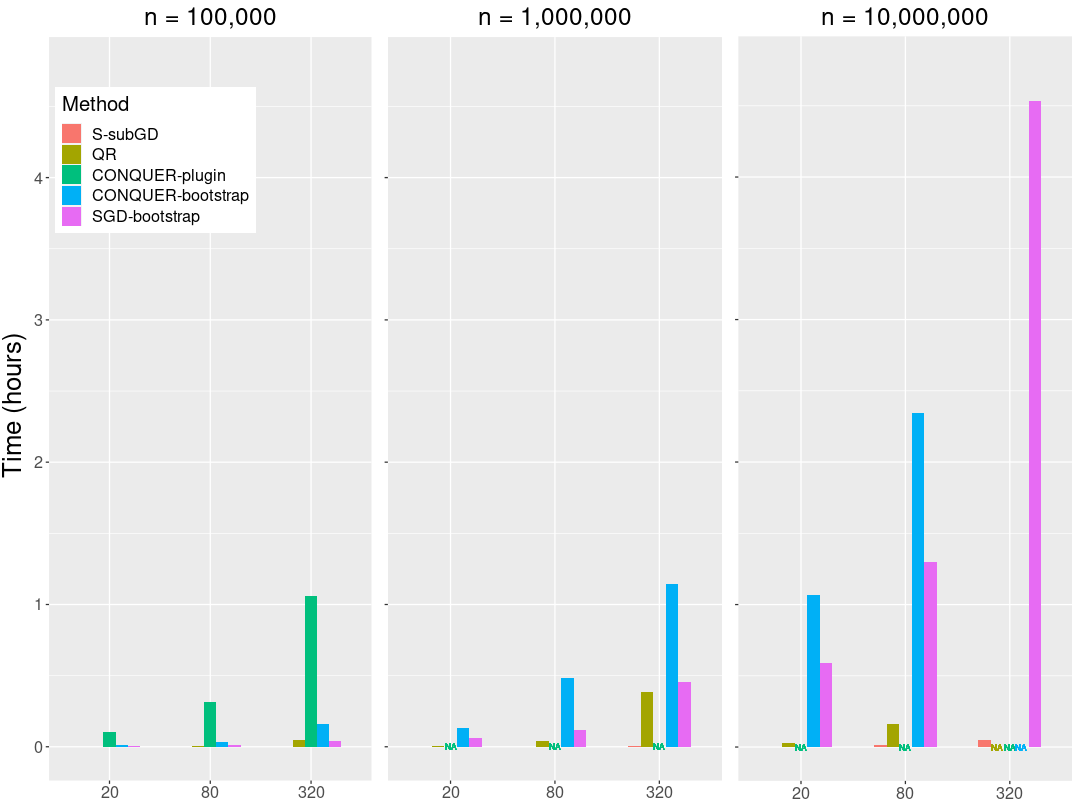
\includegraphics[width=0.7\textwidth]{fig_time.png}
%		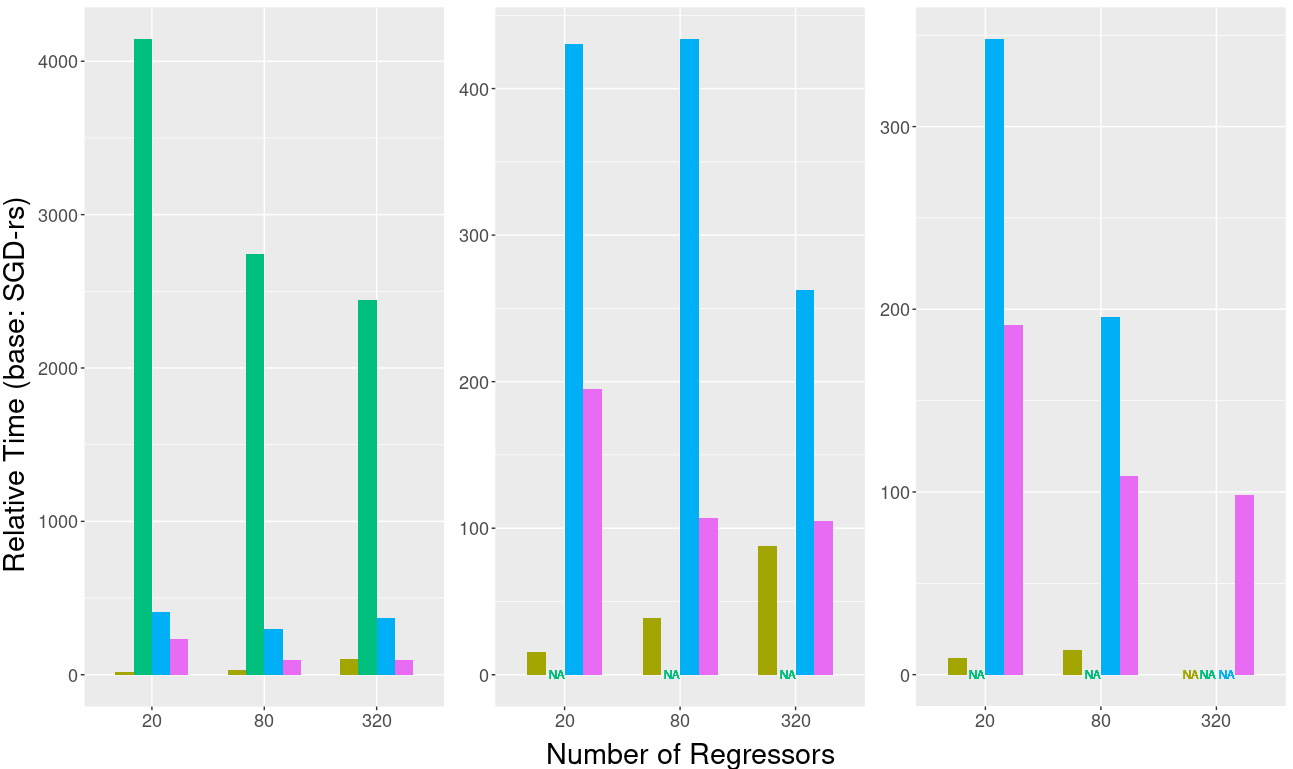
\includegraphics[width=\textwidth]{fig_rel_time.png}
	\end{figure}

Note: Observe 'NA' for several cases.
	
\end{frame}
\begin{frame}
	\begin{figure}[!htbp]
		\caption{Computation time} \label{fig:time}
		\centering
		\vskip10pt
%		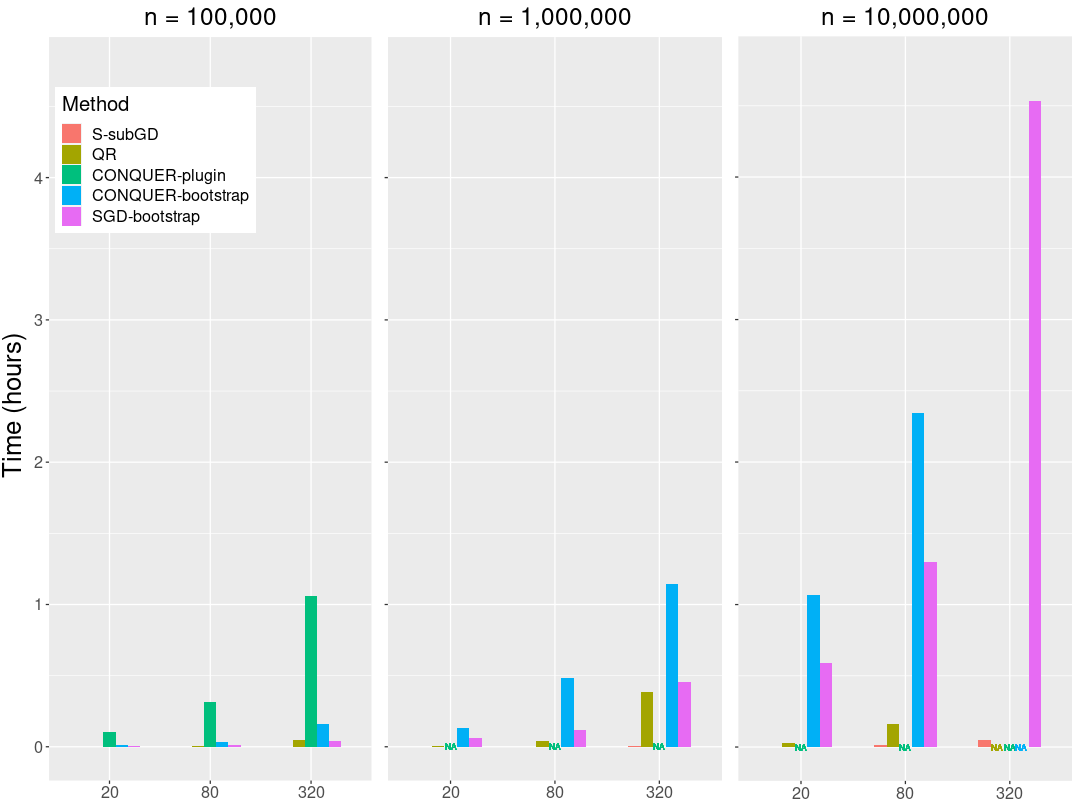
\includegraphics[width=\textwidth]{fig_time.png}
		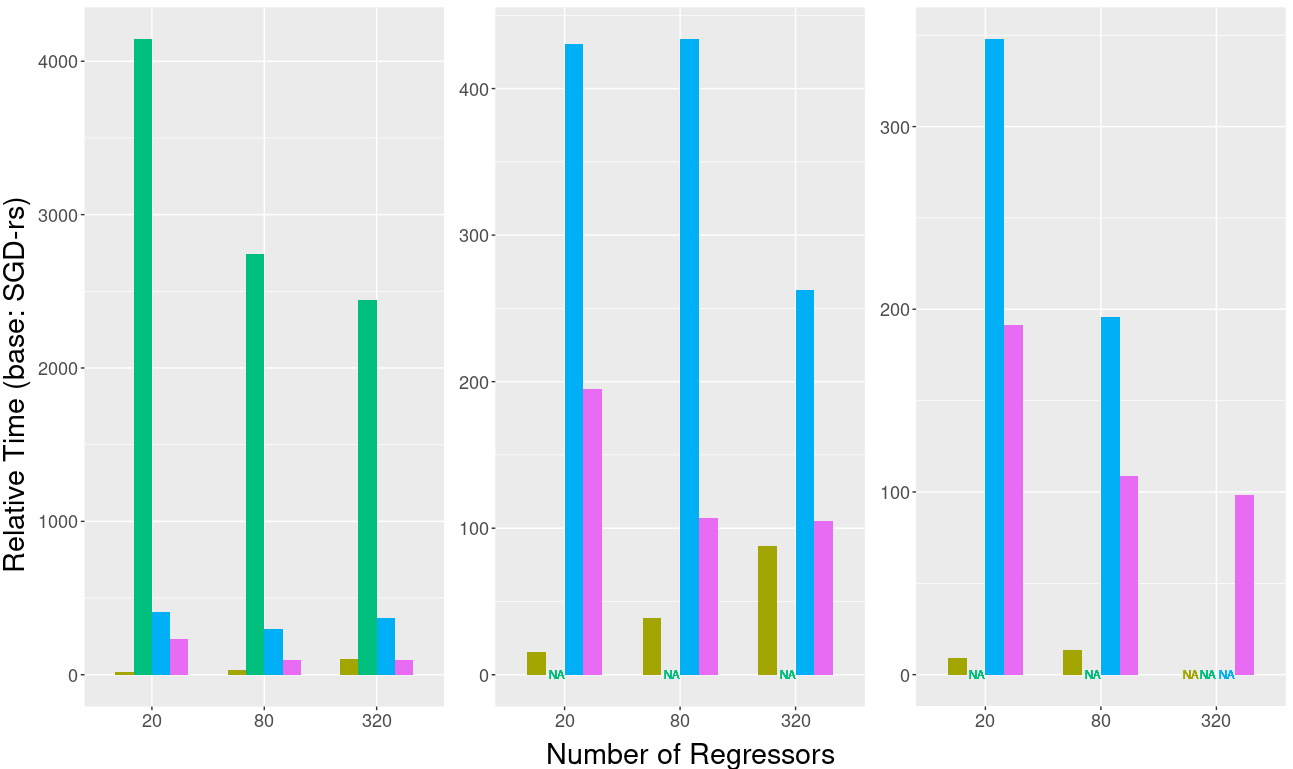
\includegraphics[width=\textwidth]{fig_rel_time.png}
	\end{figure}
	
\end{frame}

\begin{frame}
	
	\begin{figure}[!htbp]
		\caption{Coverage Rate} \label{fig:ci}
		\centering
		\vskip10pt
		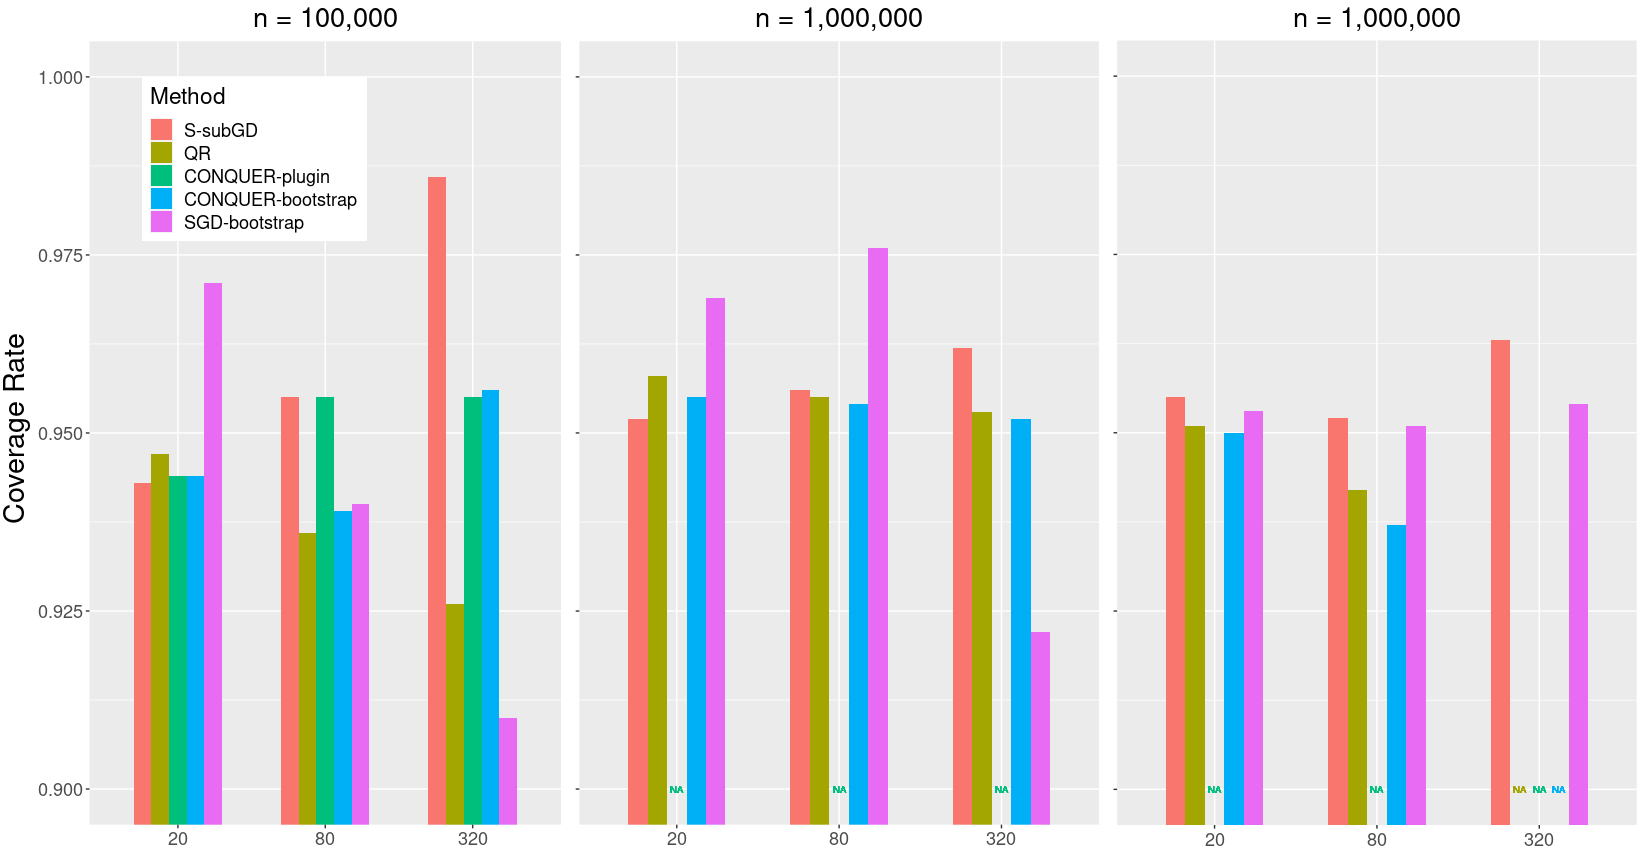
\includegraphics[width=\textwidth]{fig_coverage.png}
	%	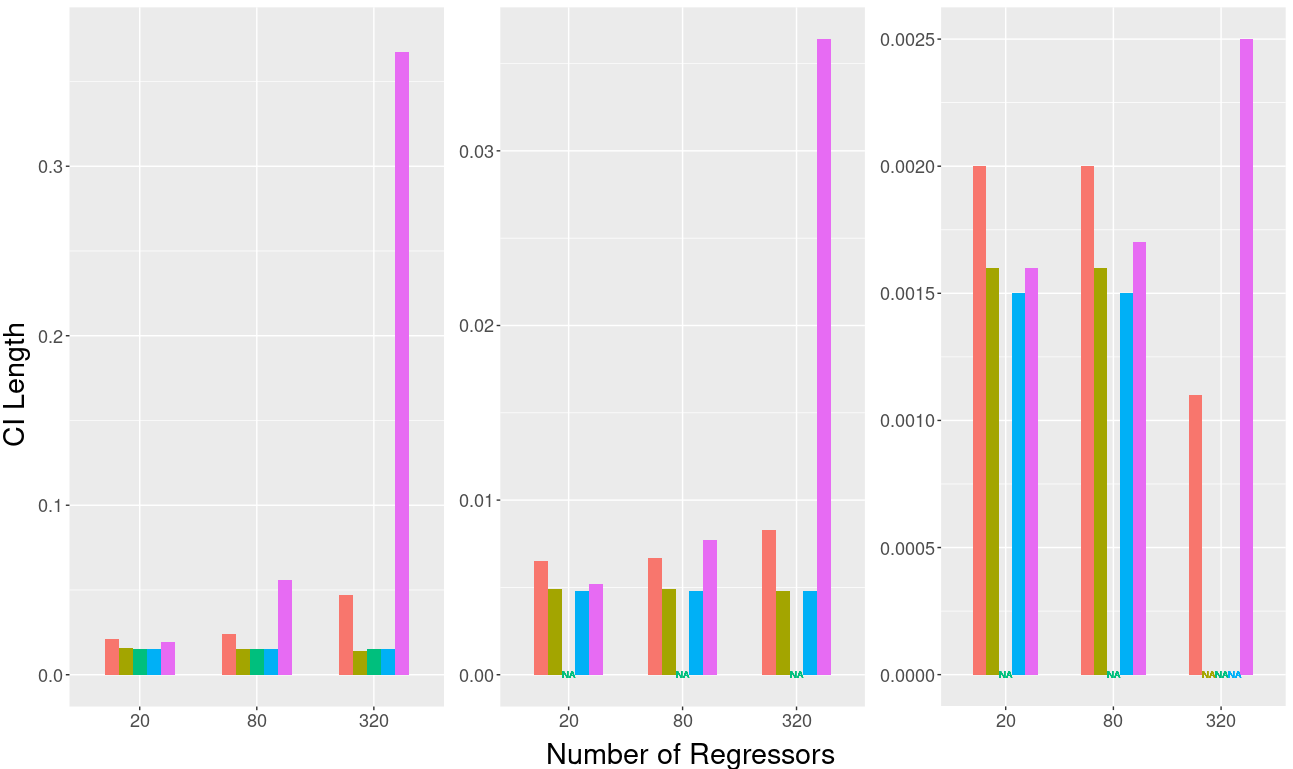
\includegraphics[width=\textwidth]{fig_ci_length.png}
	\end{figure}
	
\end{frame}


\begin{frame}
	
	\begin{figure}[!htbp]
		\caption{Confidence Interval Length} \label{fig:ci}
		\centering
		\vskip10pt
%		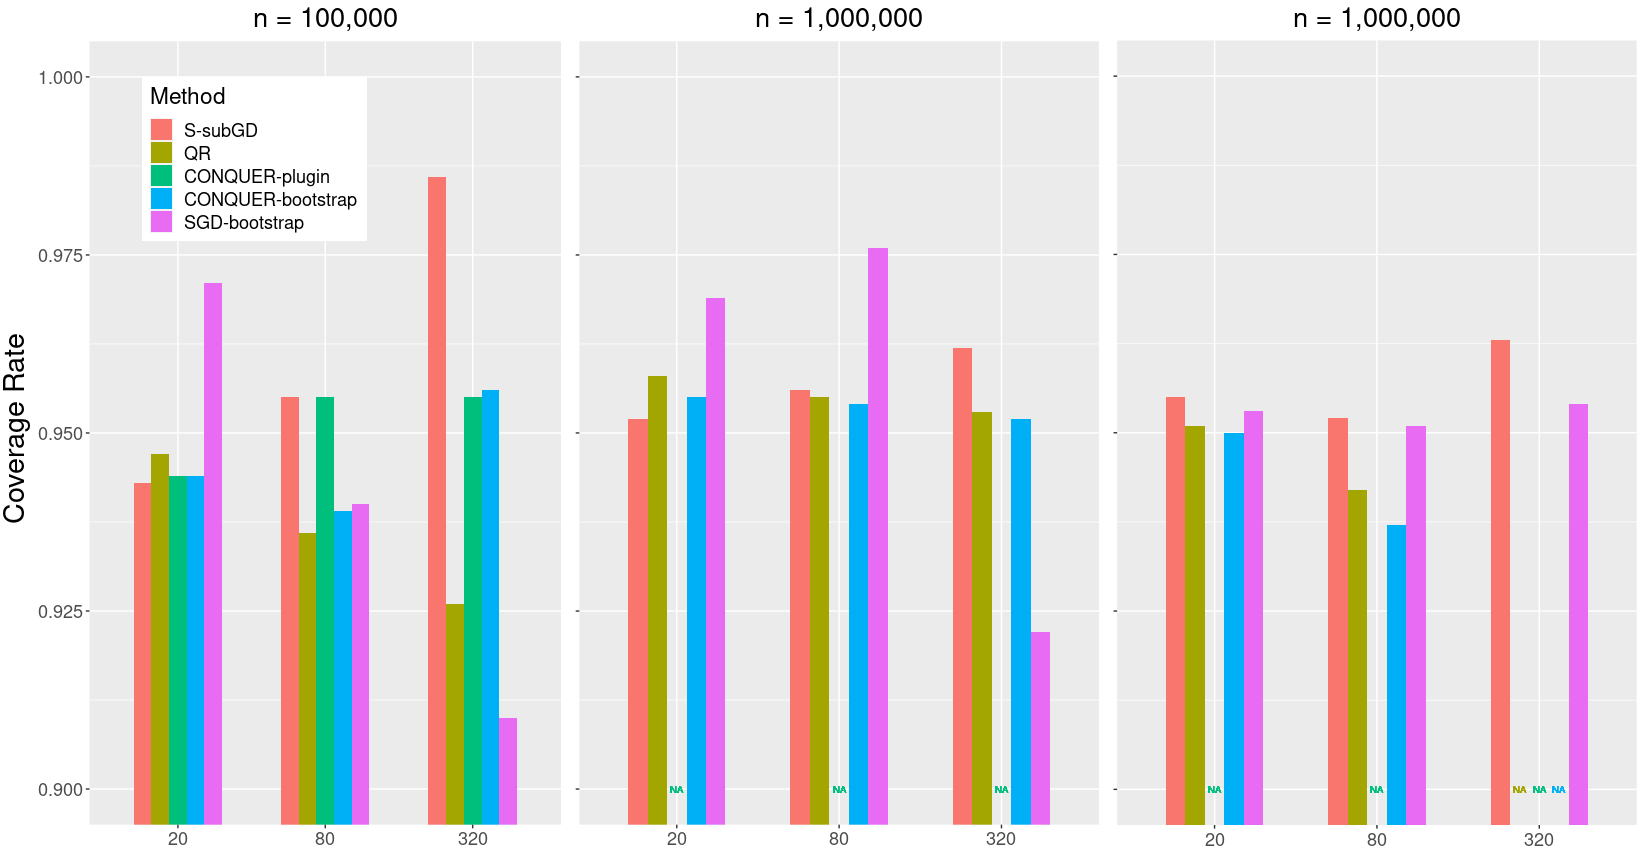
\includegraphics[width=\textwidth]{fig_coverage.png}
			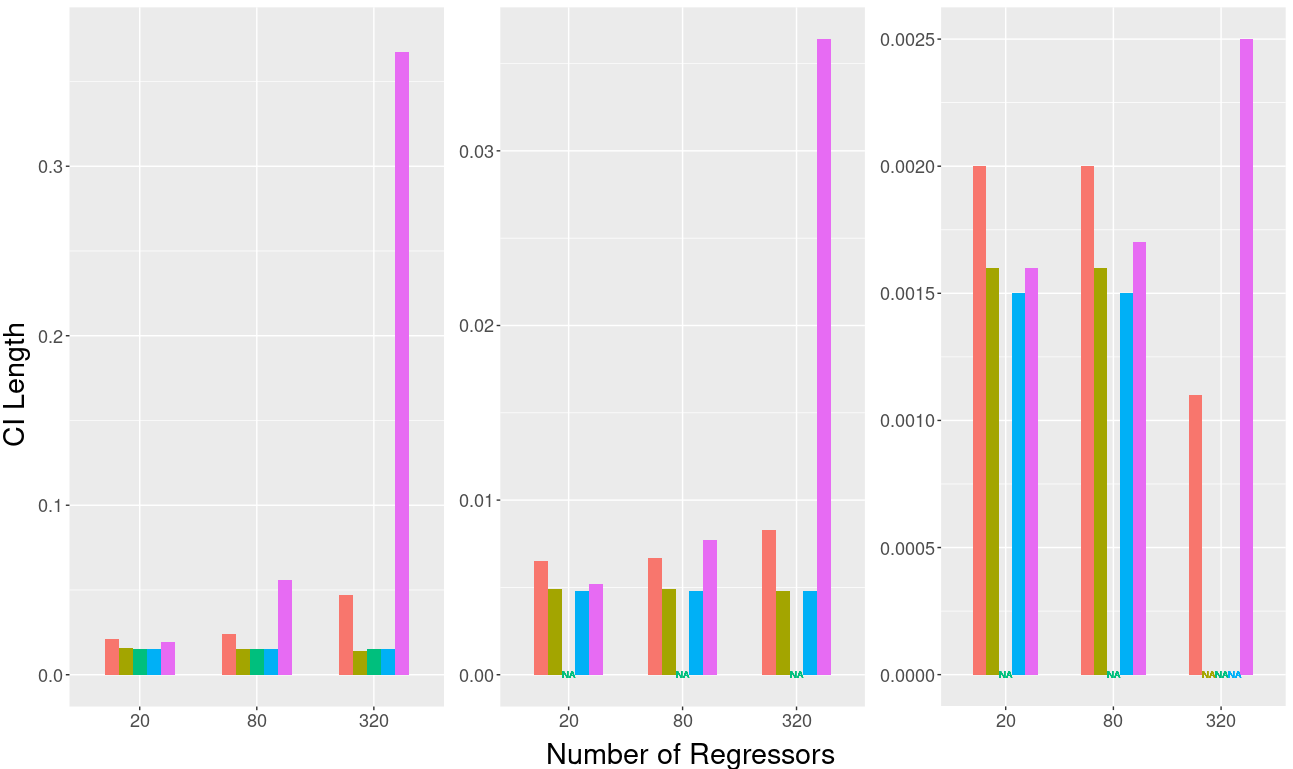
\includegraphics[width=\textwidth]{fig_ci_length.png}
	\end{figure}
	
\end{frame}


\begin{frame}
	
	\begin{table}[htb]
		\centering
		\caption{Performance of S-subGD: $n=10^7$} 
		\label{tb_SGD_rs}
		\begin{tabular}{cccc
%				S[table-format=3.2]S[table-format=1.3]S[table-format=1.4]
			}
			\hline
			{$d$} & {Time (sec.)} & {Coverage Rate} & {CI Length} \\ 
			\hline
			10 & 5.87 & 0.965 & 0.0020 \\ 
			20 & 11.05 & 0.955 & 0.0020 \\ 
			40 & 21.86 & 0.954 & 0.0020 \\ 
			80 & 43.12 & 0.952 & 0.0020 \\ 
			160 & 81.35 & 0.953 & 0.0021 \\ 
			320 & 166.40 & 0.963 & 0.0011 \\ 
			1000 & 762.16 & 0.925 & 0.0461 \\ 
			\hline
		\end{tabular}
	\end{table}
	
	
\end{frame}


%\section{Linear and Logistic Regression}
%
%\begin{frame}
%\vfill
%\centering
%\LARGE{Numerical Experiments}
%\vfill
%\end{frame}
%
%
%\begin{frame}[allowframebreaks]{Simulations: Linear Regression}
%
%
%
%The data are generated from
%\begin{align*}
%y_{t} = x_t'\beta^* + \varepsilon_t~~\mbox{for}~~t=1,\ldots,n,
%\end{align*}
%where $x_t$ is a $d$-dimensional covariate vector generated from the multivariate normal distribution $\mathcal{N} (0,I_d)$, $\varepsilon_t$ is from $N(0,1)$, and $\beta^*$ is equi-spaced on the interval $[0,1]$.
%
%%\medskip
%%This experimental design is the same as that of Zhu et al.~(2021).
%
%\medskip
%The dimension of $x$ is set to $d=5,20$.
%
%\medskip
%We consider different combination of the learning rate $\gamma_{t}=\gamma_0 t^{-a}$ by setting $\gamma_0=0.5, 1$ and $a = 0.505, 0.667$.
%
%\medskip
%The sample size set to be $n=100,000$.
%The initial value $\beta_0$ is set to be zero.
%
%\medskip
%In case of $d=20$, we burn in around 1\% of observations and start to estimate $\bar{\beta}_t$ from $t=1000$.
%Finally, the simulation results are based on $1000$ replications.
%
%\medskip
%We compare the performance of the proposed random scaling method with the state-of-the-art methods in the literature, especially the plug-in method in Chen et al. (2020) and the recursive batch-mean method in Zhu et al.~(2021).%\footnote{We are grateful to the authors of Zhu et al. (2021) for providing us their code.}
%
%\medskip
% The performance is measured by three statistics: the coverage rate, the average length of the 95\% confidence interval, and the average computation time.
%Note that the nominal coverage probability is set at 0.95.
%%Figure~\ref{fig:main-coef} shows the coverage rates and the lengths of the 95\% confidence interval for each coefficient when $d=5,\gamma_0=0.5,$ and $\alpha=0.505$, which was the step size used in  Zhu et al. (2021).
%%When we restrict to our attention to a specific method, we do not see much difference across different coefficients.
%
%\medskip
%For brevity, we focus on the first coefficient $\beta_1$ hereafter. The results are similar across different coefficients.
%
%
%\begin{figure}[htp]
%\tiny
%\caption{Linear Regression: $d \in \{5, 20\}$, $\gamma_0=0.5$, $a= 0.505$  for $\gamma_t=\gamma_0 t^{-a}$ as in Zhu et al. (2021)}\label{fig:m03-maintext}
%\centering
%\begin{tabular}{c}
%%m03
%\multicolumn{1}{c}{\underline{$d=5$}}\\
%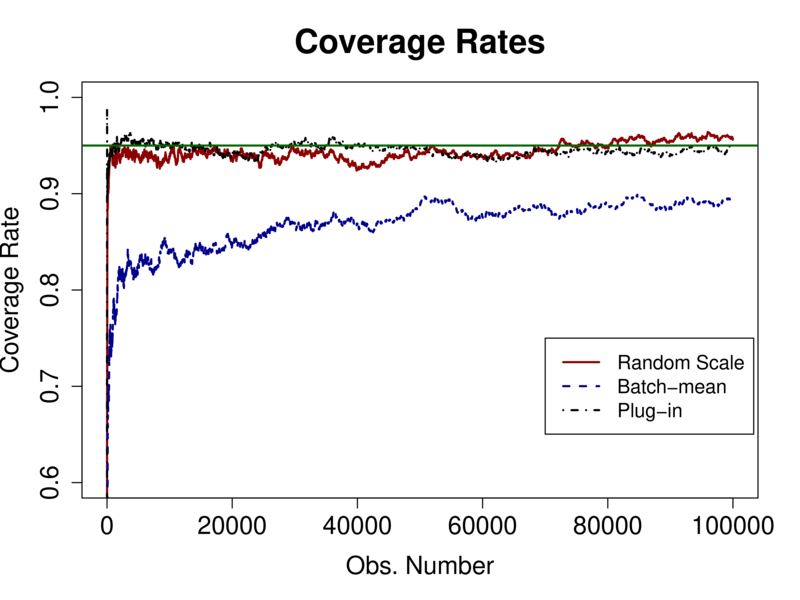
\includegraphics[scale=0.12]{figures/fig-coverage-d5-m01.png}
%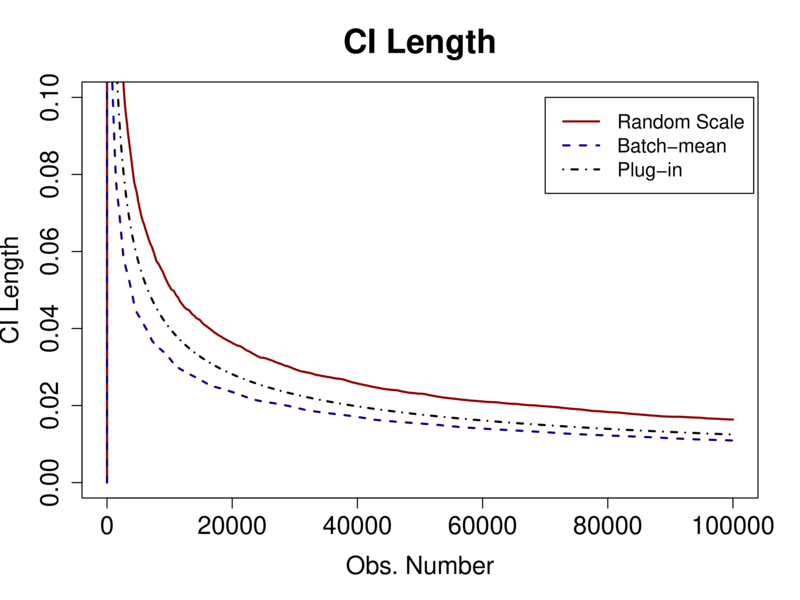
\includegraphics[scale=0.12]{figures/fig-length-d5-m01.png}
%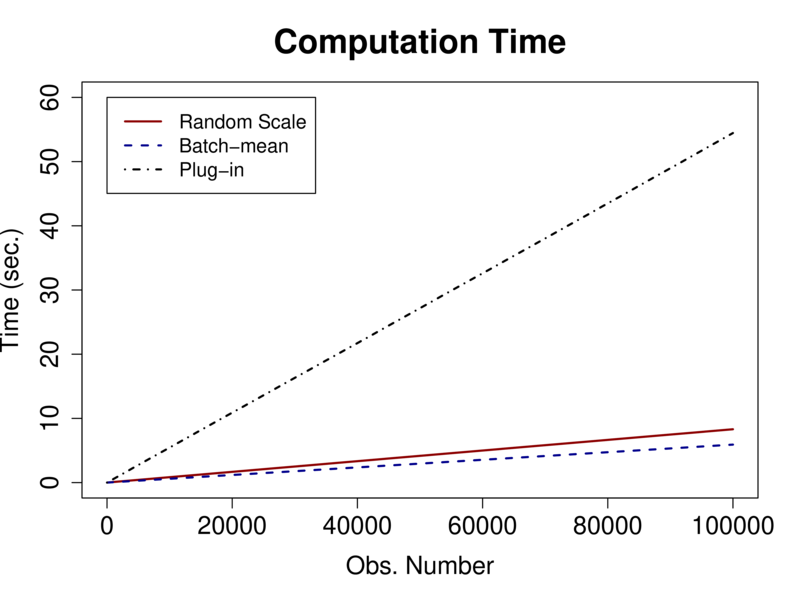
\includegraphics[scale=0.12]{figures/fig-time-d5-m01.png}\\
%\\
%\multicolumn{1}{c}{\underline{$d=20$}}\\
%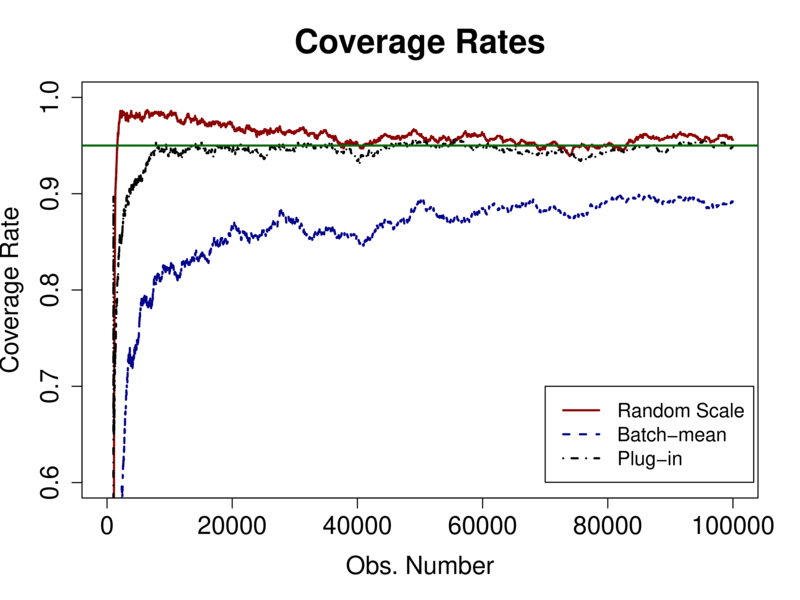
\includegraphics[scale=0.12]{figures/fig-coverage-d20-m01.png}
%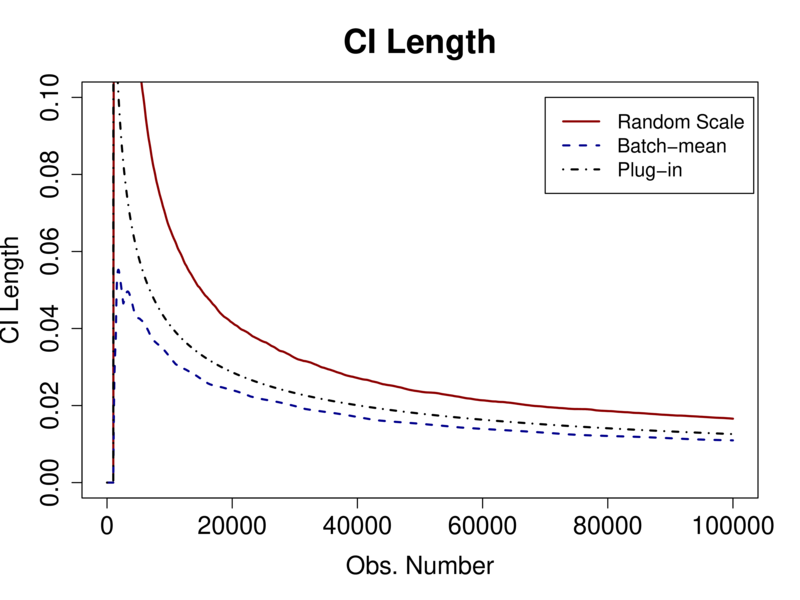
\includegraphics[scale=0.12]{figures/fig-length-d20-m01.png}
%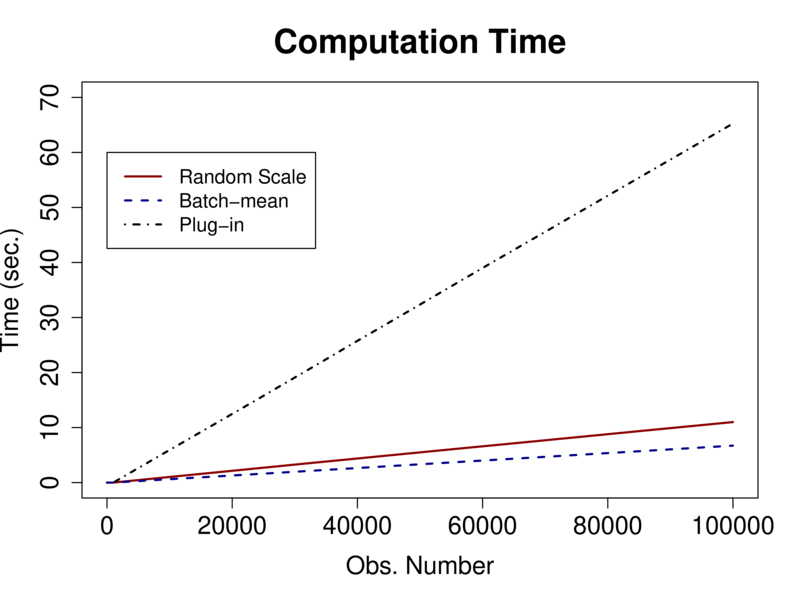
\includegraphics[scale=0.12]{figures/fig-time-d20-m01.png}\\
%\end{tabular}
%\end{figure}
%
%
%
%
%\begin{figure}[hpbt]
%\tiny
%\caption{Linear Regression: $d = 5$, $\gamma_0\in\{0.5, 1\}$, $a\in\{0.505, 0.667\}$  for $\gamma_t=\gamma_0 t^{-a}$
%}\label{fig:compare-lr-maintext}
%\centering
%\begin{tabular}{cc}
%%m03
%%\multicolumn{2}{c}{\underline{$d=5$}}\\
%{\underline{$\gamma_0=0.5, a=0.505$}} & {\underline{$\gamma_0=0.5, a=0.667$}} \\
%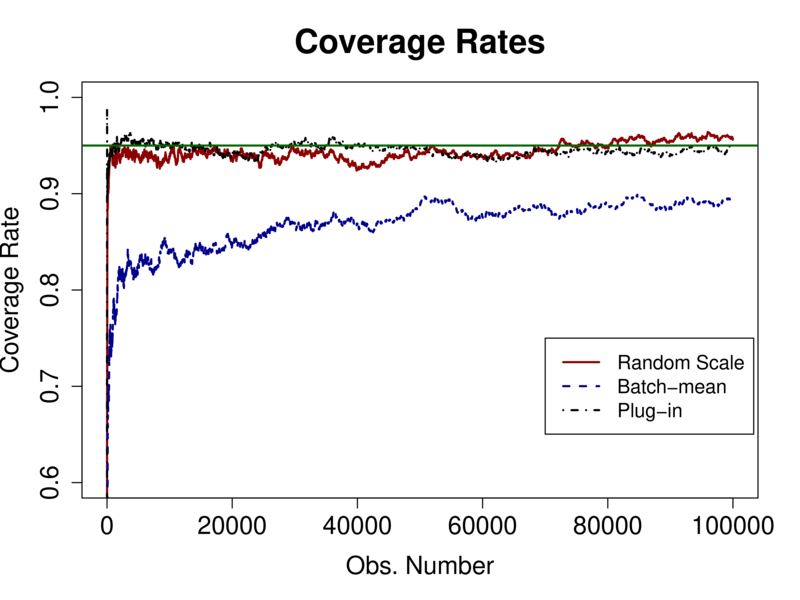
\includegraphics[scale=0.12]{figures/fig-coverage-d5-m01.png} & 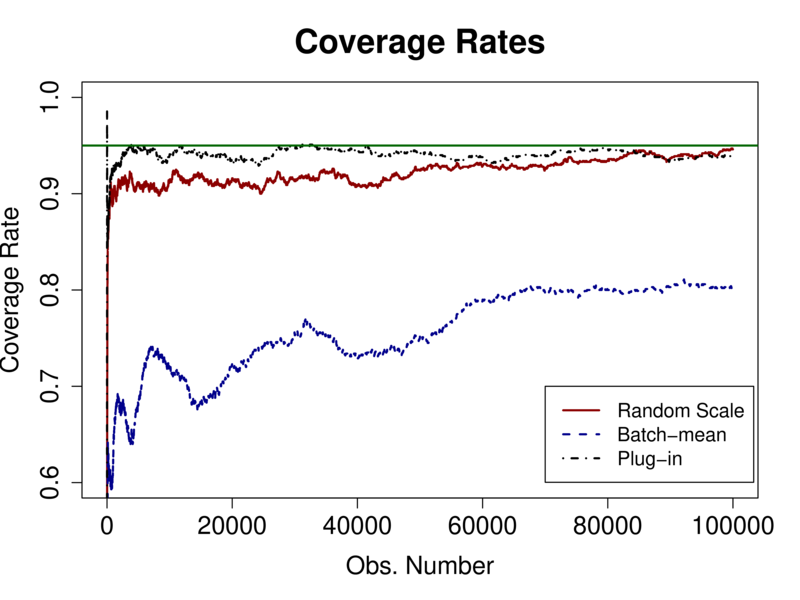
\includegraphics[scale=0.12]{figures/fig-coverage-d5-m02.png} \\
%{\underline{$\gamma_0=1, a=0.505$}} & {\underline{$\gamma_0=1, a=0.667$}}\\
% 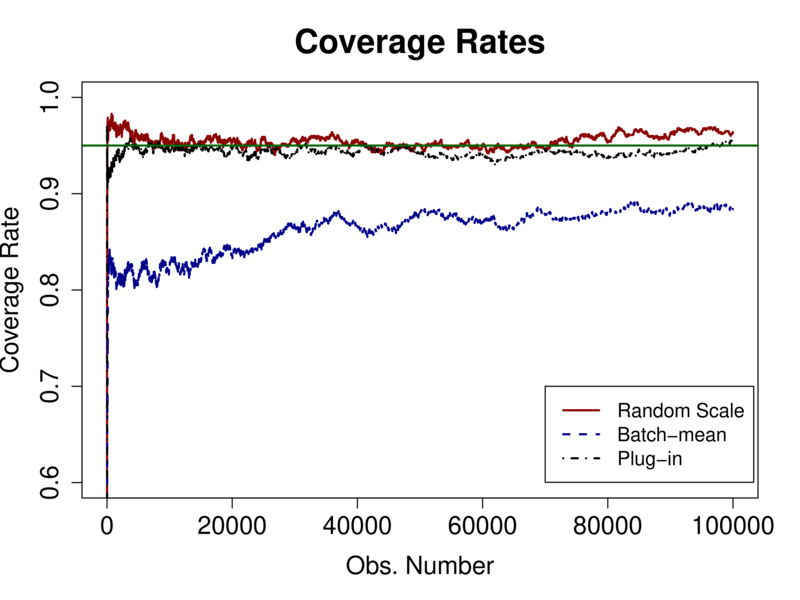
\includegraphics[scale=0.12]{figures/fig-coverage-d5-m03.png} & 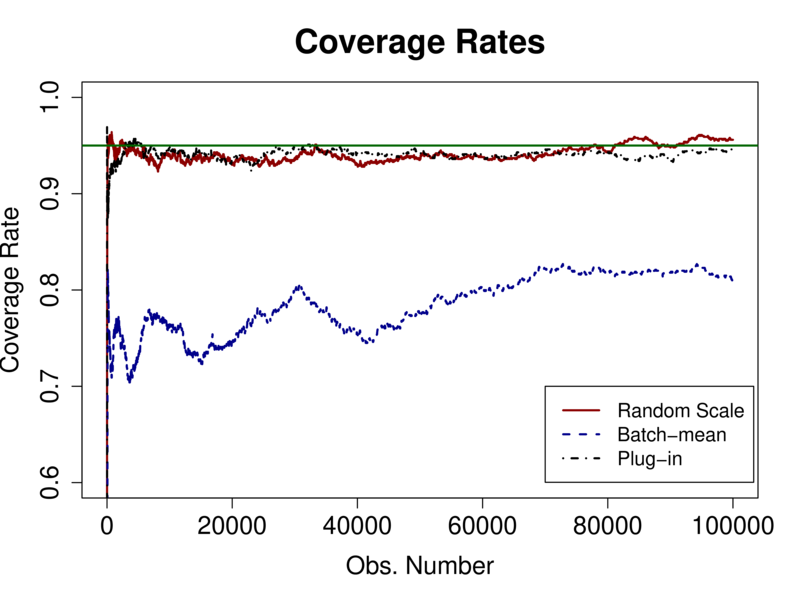
\includegraphics[scale=0.12]{figures/fig-coverage-d5-m04.png}\\
%\\
%%\multicolumn{2}{c}{\underline{$d=20$}}\\
%%{\underline{$\gamma_0=0.5, \alpha=0.505$}} & {\underline{$\gamma_0=0.5, \alpha=0.667$}}\\
%%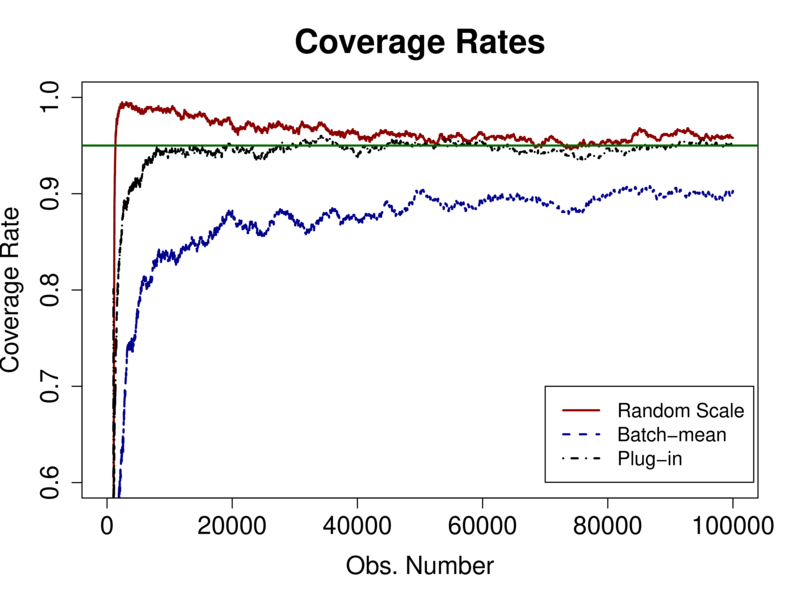
\includegraphics[scale=0.22]{figures/fig-coverage-d20-m03.png} & 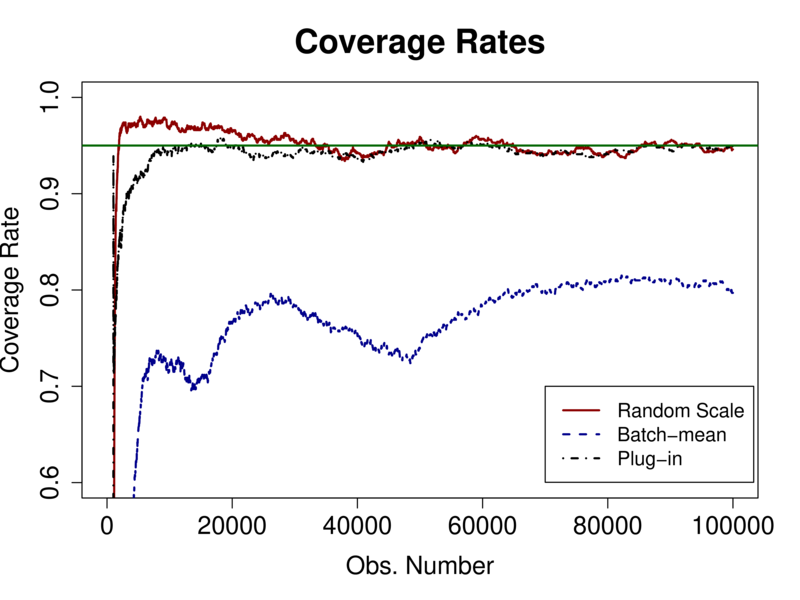
\includegraphics[scale=0.22]{figures/fig-coverage-d20-m04.png}\\
%%{\underline{$\gamma_0=1, \alpha=0.505$}} & {\underline{$\gamma_0=1, \alpha=0.667$}}\\
%%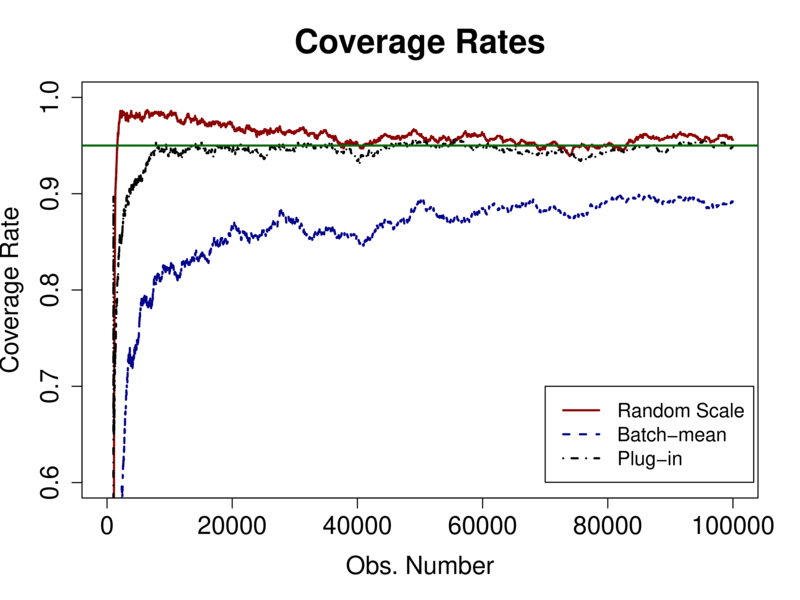
\includegraphics[scale=0.22]{figures/fig-coverage-d20-m01.png} & 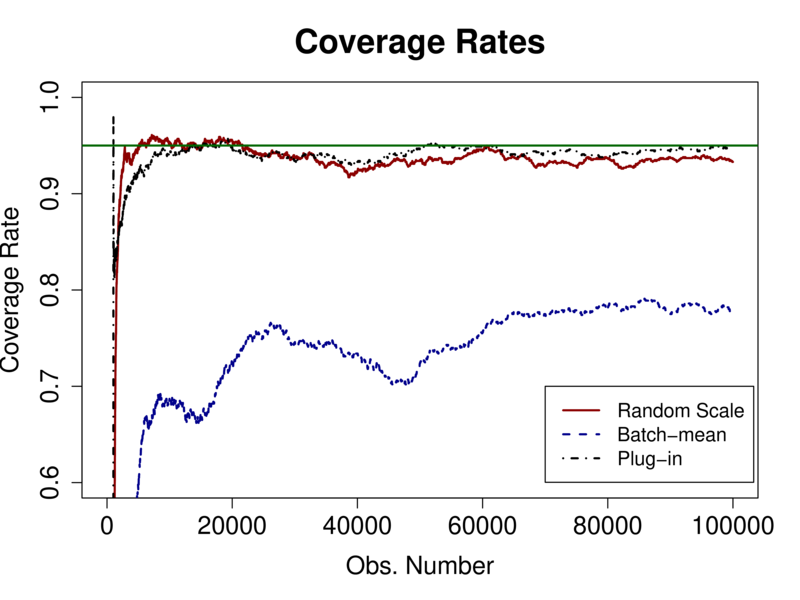
\includegraphics[scale=0.22]{figures/fig-coverage-d20-m02.png}\\
%\end{tabular}
%\end{figure}
%
%\end{frame}
%
%
%
%
%
%\begin{frame}[allowframebreaks]{Simulations: Logistic Regression}
%
%
%
%We consider the following logistic regression model:
%\begin{align*}
%y_t = 1(x_t'\beta^* - \varepsilon_t \ge 0)~~\mbox{for}~~t=1,\ldots,n,
%\end{align*}
%where $\varepsilon_t$ follows the standard logistic distribution and $1(\cdot)$ is the indicator function.
%
%\medskip
%We consider a large dimension of \(x_t\) (\(d=200\)) as well as \(d=5, 20\).
%
%\medskip
%All other settings are the same as the linear model.
%
%\framebreak
%
%\begin{table}[htbp]
%\scriptsize
%\centering
%\caption{Logistic Regression, $n=10^5$, $\gamma_0=0.5$, $a=0.505$  for $\gamma_t=\gamma_0 t^{-a}$} \label{tb:logit}
%\begin{tabular}{lccc}
%\hline
%                        &    $d=5$     &     $d=20$     &   $d=200$        \\
%\hline
% \underline{Random Scale}      \\
%Coverage               &    0.930     &     0.929      &     0.919        \\
%Length                 &    0.036     &     0.043      &     0.066   \\
%Time (sec.)            &     8.4      &      11.4      &     170.3     \\
%\hline
%\underline{Batch-mean}  \\
%Coverage               &    0.824 &     0.772      &     0.644        \\
%Length                 &    0.022     &     0.024      &     0.027       \\
%Time (sec.)            &     6.0      &       7.0      &      10.7       \\
%\hline
%\underline{Plug-in}       \\
%Coverage              &    0.953     &     0.946      &     0.944        \\
%Length                 &    0.029     &     0.035      &     0.053        \\
%Time (sec.)            &    55.2      &      66.8      &     955.0       \\
%\hline
%
%\end{tabular}
%\end{table}
%
%%\framebreak
%
%\medskip
%Overall, the simulation results are similar to those in linear regression.
%Random Scale requires more computation time than Batch-mean but is still much faster than Plug-in.
%
%\framebreak
%
%\medskip
%The computation time of Random Scale can be substantially reduced when we are interested in the inference of a single parameter. In such a case, we need to update only a single element of $\hat{V}$ rather than the whole $d\times d$ matrix.
%
%\medskip
%Random Scale can be easily scaled up to $d=800$ with only 11.7 seconds computation time when we are interested in the inference of a single parameter.
%
%%\item The performance of Random-scale is less sensitive to the choice of tuning parameters than Batch-mean.
%
%
%\begin{table}[htbp]
%\centering
%\caption{Logistic Regression: Random Scale Updating a Single Element of $\hat{V}$, $n=10^5$, $\gamma_0=0.5$, $a=0.505$  for $\gamma_t=\gamma_0 t^{-a}$} \label{tb:logit_single}
%\begin{tabular}{lccccc}
%\hline
%& $d=5$ & $d=20$ & $d=200$ & $d=500$ & $d=800$\\
%\hline
%Coverage &  0.930 & 0.929 & 0.919 & 0.927 & 0.931\\
%Length  & 0.037     & 0.043 &   0.066 & 0.133 & 0.196\\
%Time (sec.) &   5.0 &   5.3 &   6.7 &   9.7 &   11.7\\
%\hline
%\end{tabular}
%\end{table}
%
%\end{frame}
%
%
%\begin{frame}[allowframebreaks]{Simulations: Quantile Regression}
%\begin{center}
%\includegraphics[scale=0.27]{figures/Fig_qr_time.png}
%\includegraphics[scale=0.27]{figures/Fig_qr_rel_time.png}
%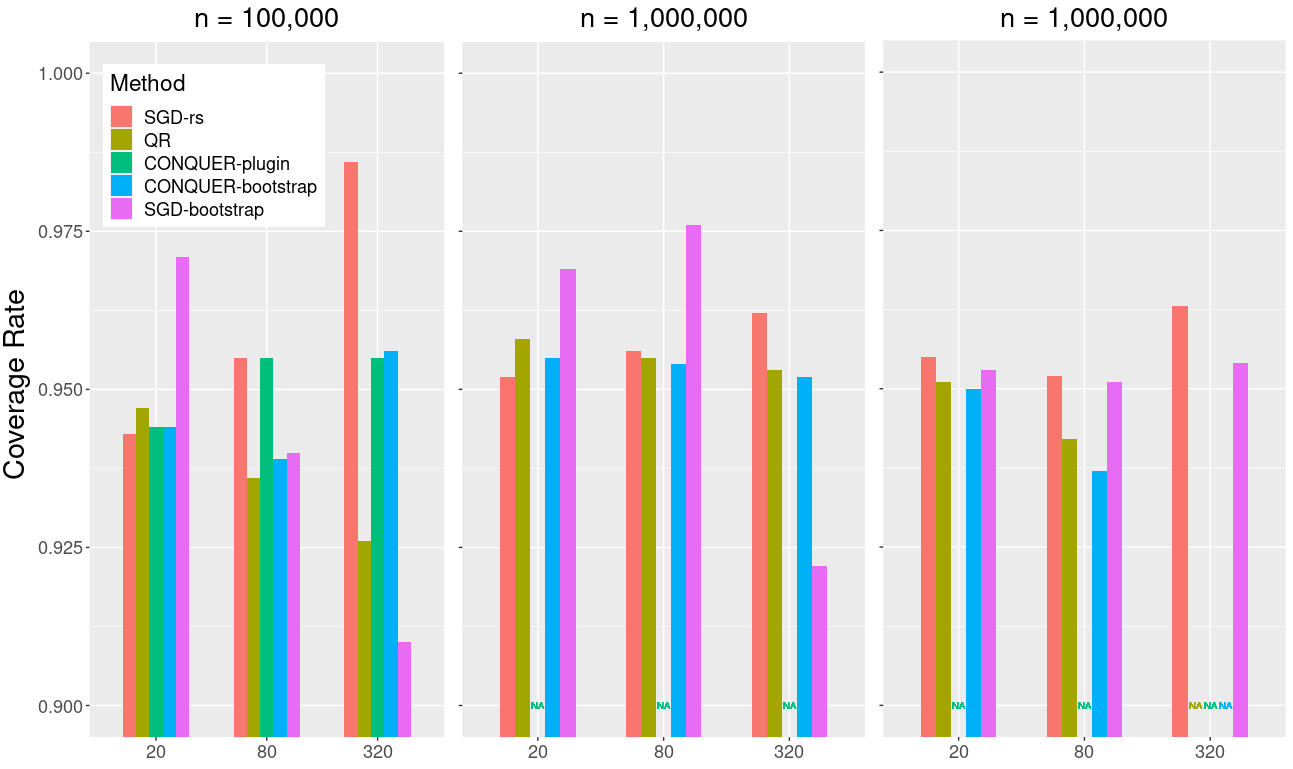
\includegraphics[scale=0.27]{figures/fig_qe_coverage}
%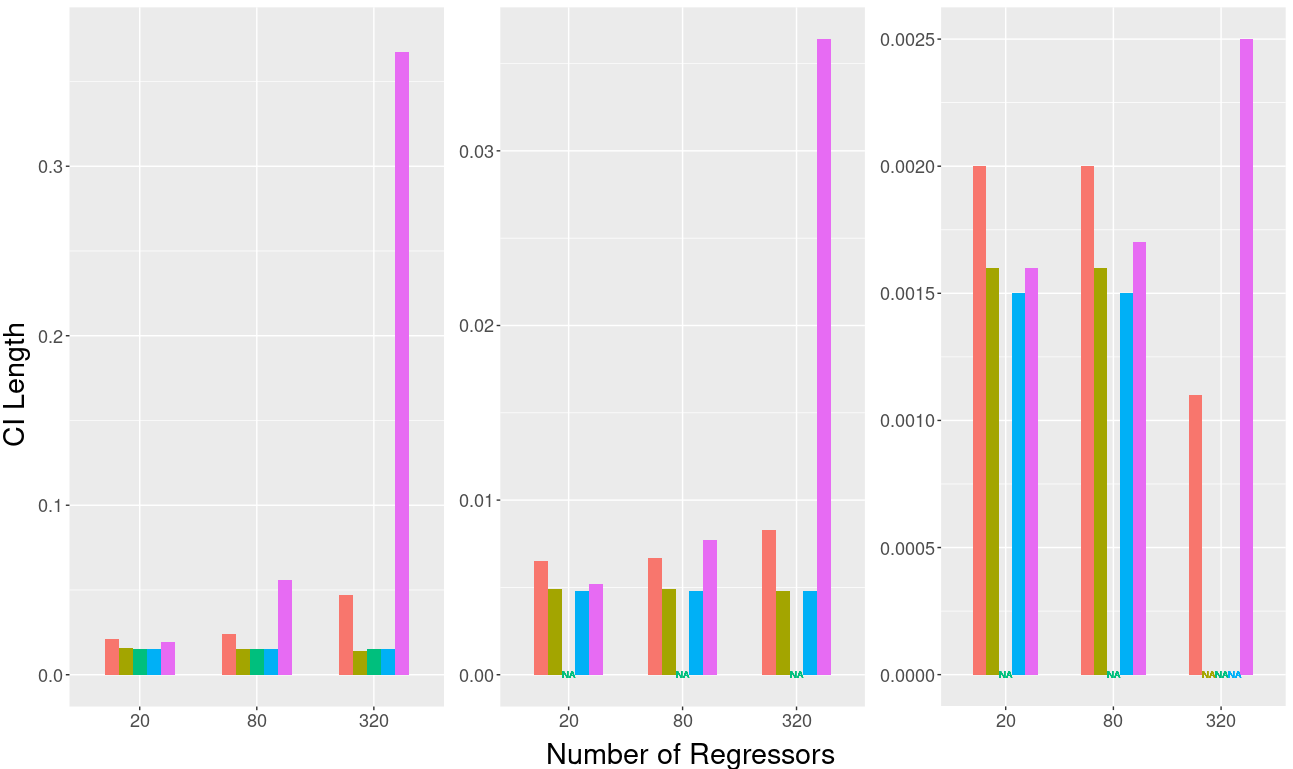
\includegraphics[scale=0.27]{figures/fig_qr_ci_length}
%\end{center}
%
%
%\end{frame}
%
%
%\begin{frame}{Application: College Premiums}
%We estimate median college premiums for male and female workers based on Hubbard (2011):
%\eqs{
%  \ln(wage_i) = \beta_0 + \beta_1 FEM_i + \beta_2 EDU_i + \beta_3 FEM_i \cdot EDU_i + \theta'X_i + \varepsilon_i,
%}where 
%\bit
%    \item $FEM_i = 1$ if Female
%    \item $EDU_i = 1$ if Some college or above
%    \item $X_i: $ $age$, $age^2$, 8 regional dummies, all interactions with $FEM_i$
%\eit
%We have 23 regressors in total.
%\medskip
%
%Data: IPUMS USA 1990, 5\% extract of the census. $n=3.6$ mil.
%
%%\begin{tiny}
%%
%%\begin{table}[ht]
%%\centering
%%\caption{Computation Time (minutes) } \label{tb:app_computation_time}
%%\begin{tabular}{crrrrrrrrrr}
%%  \hline
%% Sample Size& 10\% & 20\% & 30\% & 40\% & 50\% & 60\% & 70\% & 80\% & 90\% & 100\% \\ 
%%  \hline
%%SGD & 0.4 & 0.7 & 1.1 & 1.5 & 1.9 & 2.3 & 2.7 & 3.0 & 3.5 & 3.8 \\ 
%%QR  & 3.6 & 14.3 & 32.8 & 65.5 & 105.4 & 146.1 & 222.3 & 290.0 & 348.3 & 464.0 \\ 
%%   \hline
%%\end{tabular}
%%\end{table}
%%\end{tiny}
%
%\end{frame} 
%
\section{Application}

\begin{frame}
	\vfill
	\centering
	\LARGE{Application to College Wage Premium}
	\vfill
\end{frame}

\begin{frame}{Gender Gap in College Wage Premium}
	
	\begin{itemize}
		\item a stylized fact that the higher college wage premium for women as the major cause for attracting more women to attend and graduate from colleges than men (e.g., Goldin et al. (2006); Chiappori et al. (2009)).
		
		\item Current Population Survey (CPS) data : top coded wage issue $ \Rightarrow  $ Hubbard's (2011) quantile regression
		
		\item Our Goals:
		
		\begin{enumerate}
			\item identify (if any) the heterogeneous effects across quantiles 
			
			\item properly control other observable characteristics, such as work experience. \note{We use the data from IPUMS USA that contains several millions of workers. The main motivation of using  ultra-large datasets for wage regressions is to deal with high-dimensional regressors within a simple parametric quantile regression model. As has been crucially pointed out in the literature,  work experience is 
				an important factor in wage regressions, but is difficult to be measured precisely. One typical means of controlling for the experience is to flexibly interact workers' age with various state-level dummies, which would create over one thousand regressors, so that  a very large sample size would be desirable to obtain precise estimates. 
				But the ultra-large dataset makes most existing inference procedures for quantile regression fail to work. 
			}
			
			\item understand the trends in the college wage premium respectively for female and male
			
			\item understand the difference in gender trends in the college wage premium.
			
		\end{enumerate}
		
	\end{itemize}


\end{frame}

\begin{frame}[allowframebreaks]{Data}
	\begin{itemize}
		\item We use the samples over six different years (1980, 1990, 2000-2015) from IPUMS USA at \url{https://usa.ipums.org/usa/}. 
		
		\item
		In the years from 1980 to 2000, we use the 5\% State sample which is a 1-in-20 national random sample of the population. 
		In the remaining years, we use the American Community Survey (ACS) each year. 
		
		\item The sampling ratio varies from 1-in-261 to 1-in-232 in 2001-2004, but it is set to a 1-in-100 national random sample of the population after 2005. 
		
		\item
		To balance the sample size, we bunch the sample every 5 year after 2001. 
		
		\item We restrict our sample to $White$, $18 \le Age \le 65$,  and $Wage \ge \$62$, which is a half of minimum wage earnings in 1980 ($\$3.10 \times 40 \mbox{hours} \times 1/2$). 
		
		\item
		$Wage$ denotes the implied weekly wage that is computed by dividing yearly earnings by weeks worked last year. 
		\item
		We only consider full-time workers who worked more than 30 hours per week.
		
		\item
		Then, we compute the \textit{real} wage using the personal consumption expenditures price index (PCEPI) normalized in 1980. 
		
		\item
		The data cleaning leaves us with 3.6-4.7 million observations besides 2001-2005, where we have around 2.5 million observations.
		
		\item  $Educ$ denotes an education dummy for some college or above. 
		
		\item For control, we use 12 age group dummies with a four-year interval, 51 states dummies (including D.C.), and their interactions.
		The model contains 1226 covariates in total.
		We also add 4 additional year dummies for the 5-year combined samples after 2001. 
		

	\end{itemize}
\end{frame}

\begin{frame}
	
	\begin{table}[ht]
		\caption{Summary Statistics} \label{tb:summary_stat}
		\centering
		\begin{tabular}{crcccc}
			\hline
			Year & Sample Size & $\mathbb E(F$) & $\mathbb E(Edu$) & $\mathbb E(Edu|M$) & $\mathbb E(Edu|F$) \\ 
			\hline
			1980      & 3,659,684 & 0.390 & 0.433 & 0.444 & 0.416 \\ 
			1990      & 4,192,119 & 0.425 & 0.543 & 0.537 & 0.550 \\ 
			2000      & 4,479,724 & 0.439 & 0.600 & 0.578 & 0.629 \\ 
			2001-2005 & 2,493,787 & 0.447 & 0.642 & 0.619 & 0.670 \\ 
			2006-2010 & 4,708,119 & 0.447 & 0.663 & 0.631 & 0.701 \\ 
			2011-2015 & 4,542,874 & 0.447 & 0.686 & 0.646 & 0.735 \\ 
			\hline
		\end{tabular}
	\end{table}
	
			\note{The table confirms that female college education has increased substantially over the years and female workers received more college education than male workers since 1990. }
	
\end{frame}

\begin{frame}
	
	\bigskip
	
	\begin{figure}[!h]
		\centering
		\caption{College Wage Premium: %Model 3 with 
			Combining 5-Year Data %. Full-time
		}
	\bigskip
			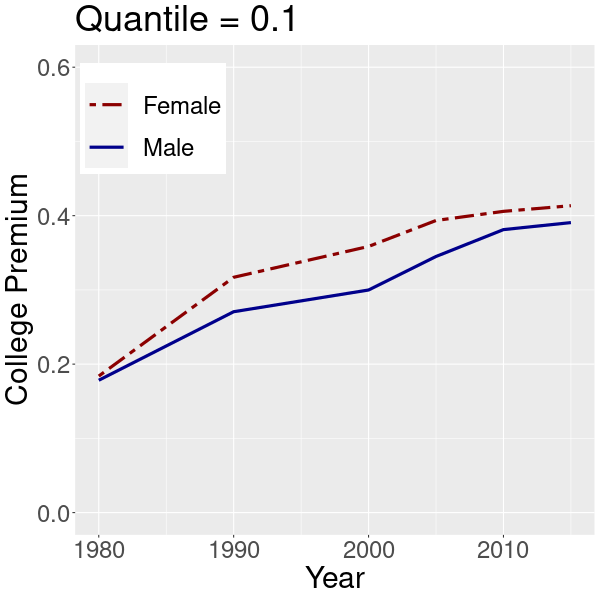
\includegraphics[width=0.3\textwidth]{chart_1_03_FullT_5yr.png}  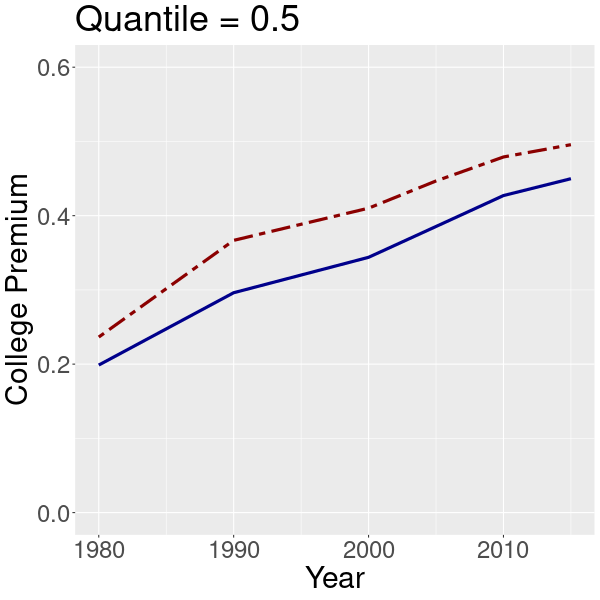
\includegraphics[width=0.3\textwidth]{chart_5_03_FullT_5yr.png} 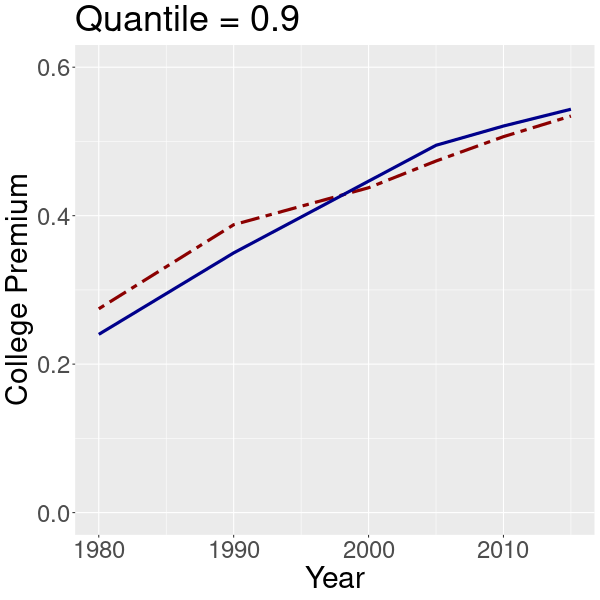
\includegraphics[width=0.3\textwidth]{chart_9_03_FullT_5yr.png} 
			
	\end{figure}
	
\end{frame}

\begin{frame}
	
	\begin{table}[htb]
		\centering
		\small
		\caption{College Wage Premium: $\tau=0.5$}\label{tb:median_5yr_full}
		\begin{tabular}{ccccc}
			\hline
			Year & Female & Male & Difference & Time (min.) \\ 
			\hline
			\underline{$\tau = 0.5$}\\
			1980 & 0.2365 & 0.1988 & 0.0377 & 29.4 \\ 
			& [0.2294,0.2435] & [0.1945,0.2030] & [0.0291,0.0463] &  \\ 
			1990 & 0.3667 & 0.2962 & 0.0705 & 34.2 \\ 
			& [0.3603,0.3732] & [0.2942,0.2982] & [0.0634,0.0777] &  \\ 
			2000 & 0.4101 & 0.3439 & 0.0662 & 36.7 \\ 
			& [0.4056,0.4146] & [0.3372,0.3506] & [0.0552,0.0772] &  \\ 
			2001-2005 & 0.4468 & 0.3854 & 0.0613 & 20.2 \\ 
			& [0.4369,0.4567] & [0.3765,0.3944] & [0.0554,0.0673] &  \\ 
			2006-2010 & 0.4791 & 0.4271 & 0.0520 & 47.7 \\ 
			& [0.4748,0.4834] & [0.4174,0.4368] & [0.0454,0.0585] &  \\ 
			2011-2015 & 0.4957 & 0.4498 & 0.0458 & 46.0 \\ 
			& [0.4887,0.5027] & [0.4455,0.4542] & [0.0348,0.0568] &  \\ 
			\hline
		\end{tabular}

	\end{table}
	
	
\end{frame}

\section{Conclusion}

\begin{frame}{Conclusion} 
	\begin{itemize}
		
		\item We provide a new scalable on-line inference method for Quantile Regression with ``ultra-large" sample sizes. 
		
		\item Fast + small memory cost
		
		\item Potential Extensions:
		
		\begin{itemize}
			
			\item cluster robust inference
			
			\item high-dimensional settings and penalized estimation like Lasso.
			
			\item more sophisticated random scaling
			
			
			
		\end{itemize}
		
		
	\end{itemize} 
\end{frame}

\fm{
\vskip30pt
\centering
   
\includegraphics[scale=1]{figures/thankyou.jpg}
}

\end{document}


